\documentclass[10pt]{beamer}
\usepackage[T1]{fontenc}
\usepackage{hyperref}
\usepackage[utf8]{inputenc}
\usepackage[english]{babel}
\usepackage{amsmath}
\usepackage{amsthm}
\usepackage{amssymb}
\usepackage{amsfonts}
\usepackage{mathtools}
\usepackage{booktabs}
\usepackage{caption}
\usepackage{graphicx}
\usepackage{float}
\usepackage{multirow}
\usepackage{braket}
\usepackage{tikz}
\usepackage{qcircuit}
\usepackage{blindtext}
\usepackage{scrextend}

\usetheme[progressbar=frametitle]{metropolis}
\metroset{block=fill}
\setbeamertemplate{frame numbering}[fraction]

\title{A study of the stochastic Saltzman-Maasch model for climate dynamics in Pleistocene}
\author{Giovanni Varutti}

\begin{document}

\begin{frame}
	\maketitle
\end{frame}

\begin{frame}{Index}
	\tableofcontents
\end{frame}

\section{Deterministic model}

\begin{frame}{The Saltzman-Maasch model}
	The model explains central features of the glacial cycles observed in the 
	climate record of the Pleistocene Epoch.

	\[
		\begin{cases}
			\dot{X} = -X -Y -vZ \\ 
			\dot{Y} = -pZ + rY -sY^2 -Y^3 \\
			\dot{Z} = -q(X+Z)
		\end{cases}
	\]

	The state variables $X, Y, Z$ represent the anomalies (deviations
	from long-term averages) of
	\begin{itemize}
		\item $X$: the total continental ice mass
		\item $Y$: the atmospheric $\text{CO}_2$ concentration
		\item $Z$: the the mean temperature of the North Atlantic Deep Water
	\end{itemize}
\end{frame}

\begin{frame}{Deterministic Equilibria}
	The model possesses the equilibrium $E_0 = (0, 0, 0)$, for all the parameter values.
	Other equilibria points $E = ( X, Y, Z)$ can be found imposing:
	\[
		\begin{cases}
			-X -Y -vZ = 0 \\ 
			-pZ + rY -sY^2 -Y^3 = 0 \\
			-q(X+Z) = 0 \implies X = -Z
		\end{cases}
	\]
	which leads to the non-trivial equilibrium points expression:
	\[
	E_{1,2} = \left(-\frac{Y_{1,2}}{1-v}, \ Y_{1,2}, \ \frac{Y_{1,2}}{1-v}\right), \quad Y_{1,2} = -\frac{s}{2} \pm \sqrt{r + \frac{s^2}{4} - \frac{p}{1-v}}
	\]
	The parameter $r$ is used as control and bifurcation parameter, fixing the others: $p = 1, q = 2.5, v = 0.2, s = 0.6$.
	Within this framework:
	\[
	E_{1,2} = \left(-1.25Y_{1,2}, \ Y_{1,2}, \ 1.25Y_{1,2} \right), \quad Y_{1,2} = -0.3 \pm \sqrt{r - 1.16} \ \ .
	\]
\end{frame}

\begin{frame}{Phase Portraits}
	\begin{figure}
		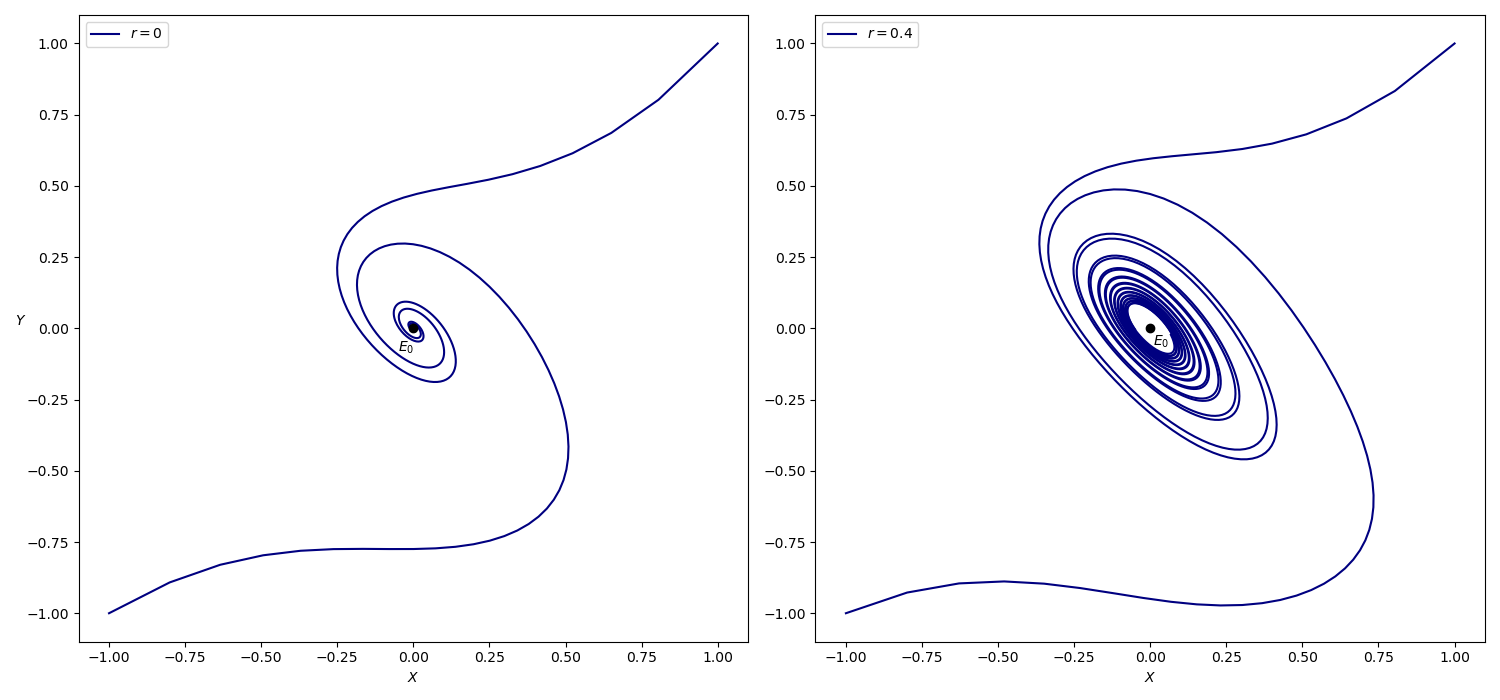
\includegraphics[width=0.82\textwidth, height=0.7\textheight,keepaspectratio]{./figures_2/r0-0.4-noiseless-trajectories.png}
		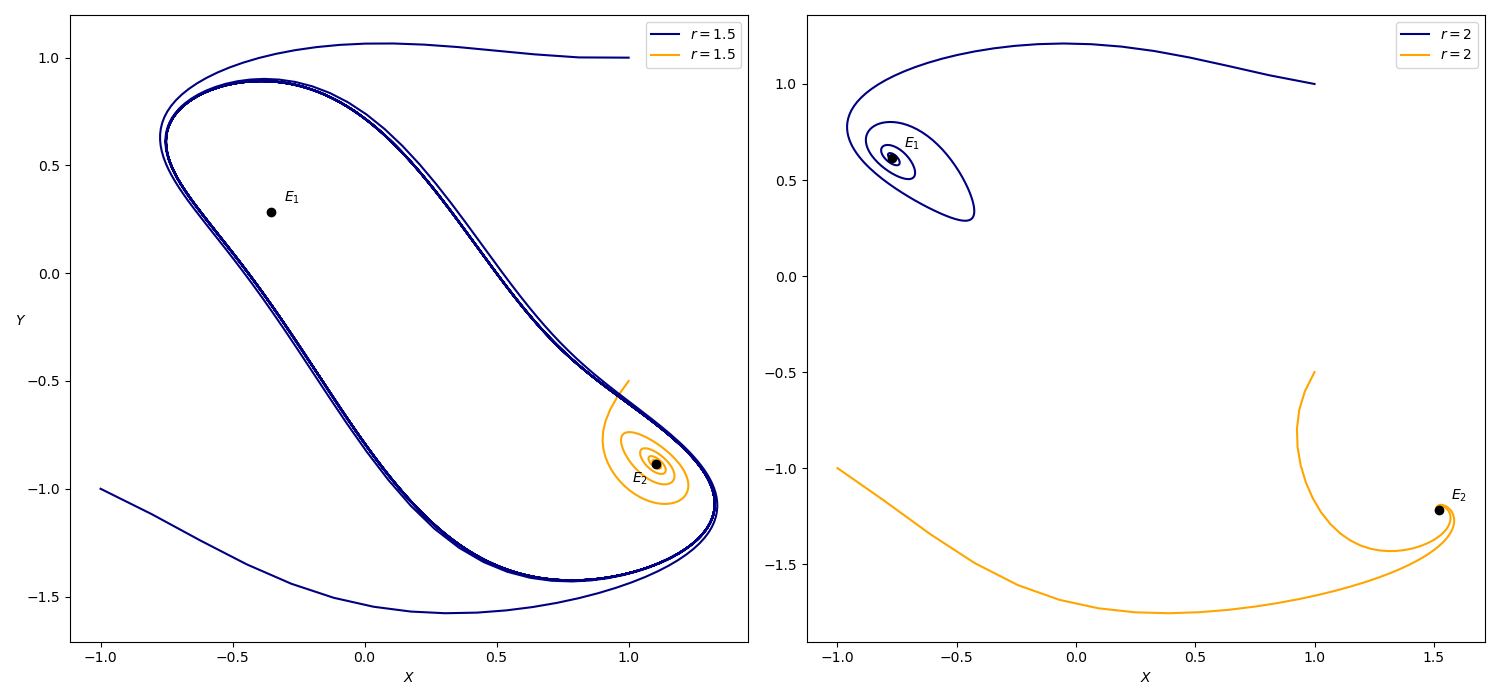
\includegraphics[width=0.82\textwidth, height=0.7\textheight,keepaspectratio]{./figures_2/r1.5-2-noiseless-trajectories.png}
	\end{figure}
\end{frame}

\begin{frame}{Attractors: monostability and bistability regions}
	\begin{figure}
		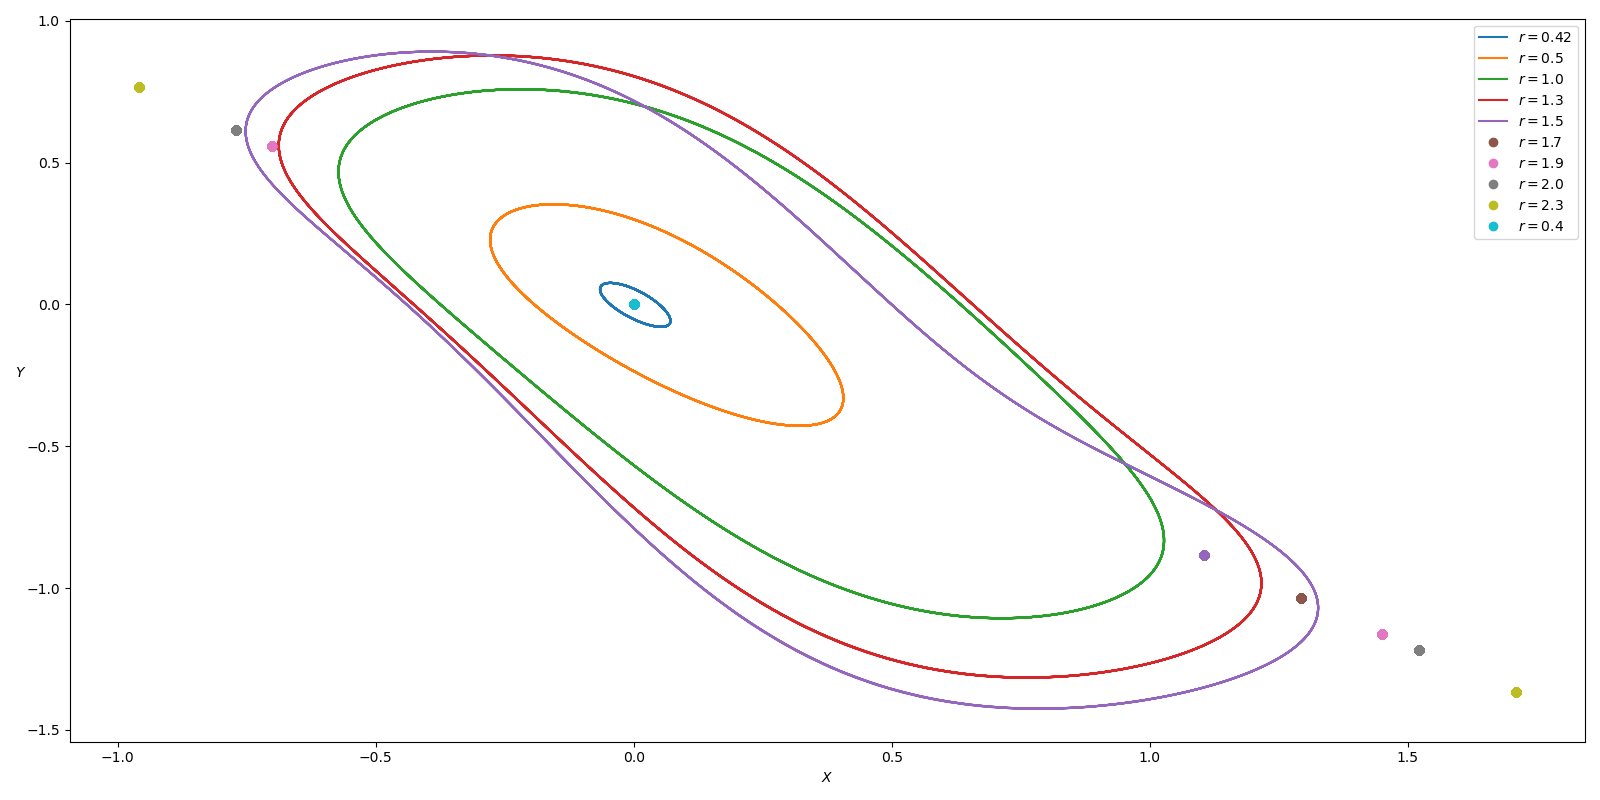
\includegraphics[width=\textwidth, height=\textheight,keepaspectratio]{./figures_2/noiseless-attractors.png}
	\end{figure}

	For $r<0.42$: monostability in $E_0$.
	Around $r\approx 0.42$: bifurcation point and periodic cycles as attractors.
	Around $r\approx1.5$, bistability with periodic cycles and $E_2$.
	Around $r\approx1.7$ periodic cycles loss and monostability (brown point).
	For $r>1.9$, bistability with $E_1$ and $E_2$.
\end{frame}

\begin{frame}{Time Behavior and Histograms}
	\begin{figure}
		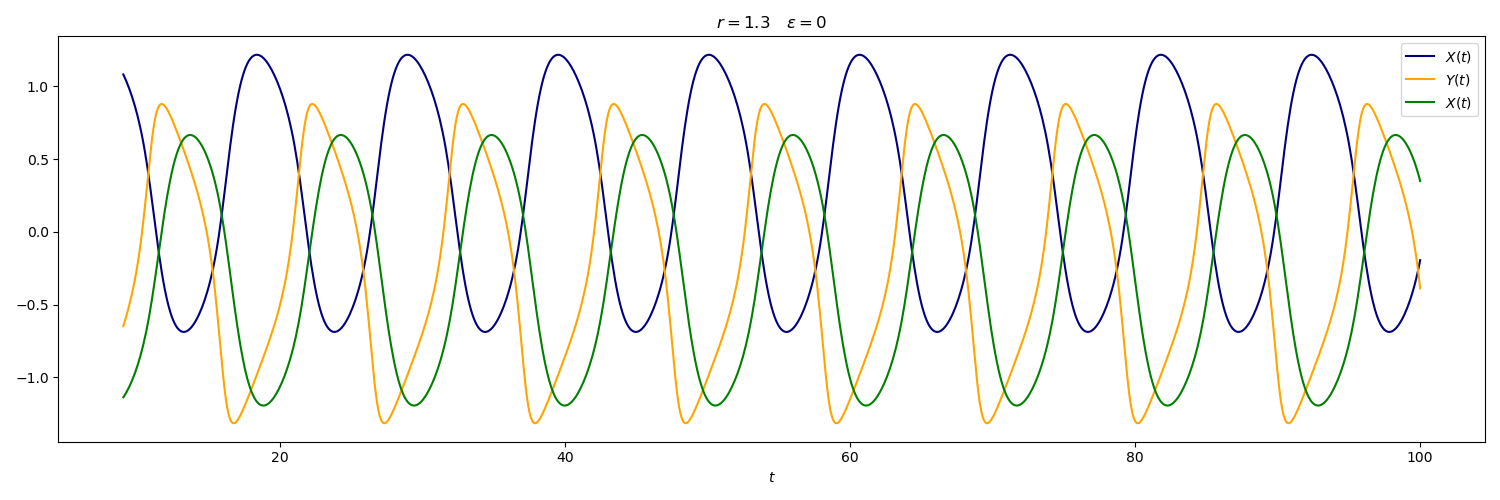
\includegraphics[width=\textwidth, height=0.52\textheight,keepaspectratio]{./figures_2/r1.3-noiseless-time-trajectories.png}
		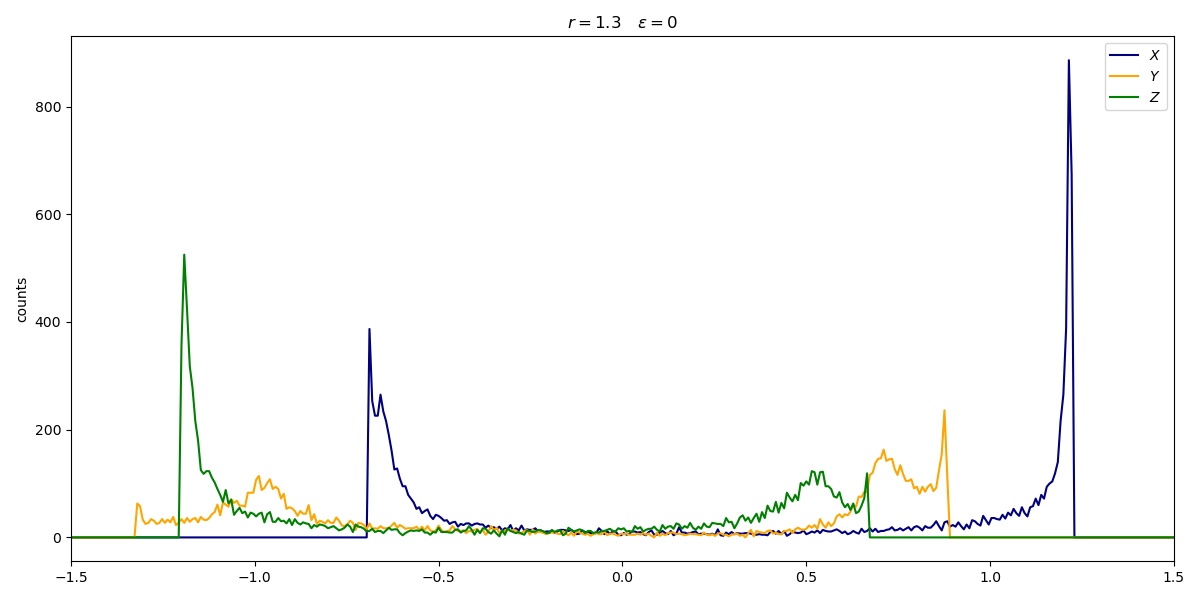
\includegraphics[width=\textwidth, height=0.52\textheight,keepaspectratio]{./figures_2/r1.3-noiseless-hist-2.png}
	\end{figure}
\end{frame}

\begin{frame}{Time Behavior and Histograms}
	\begin{figure}
		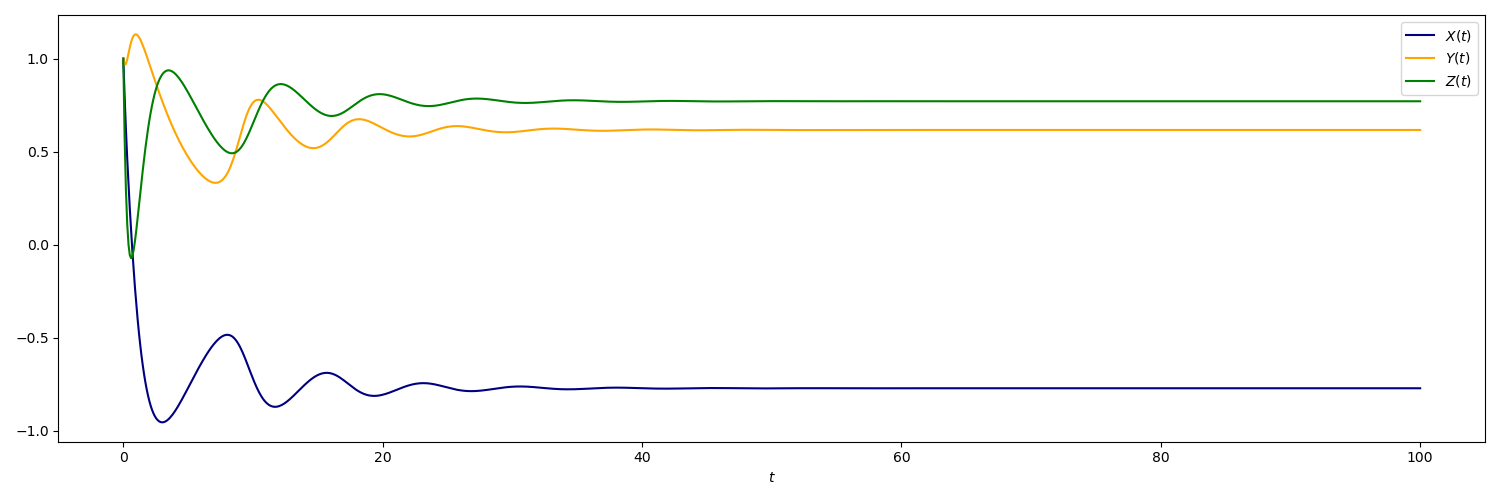
\includegraphics[width=\textwidth, height=0.52\textheight,keepaspectratio]{./figures_2/r2-noiseless-time-trajectories.png}
		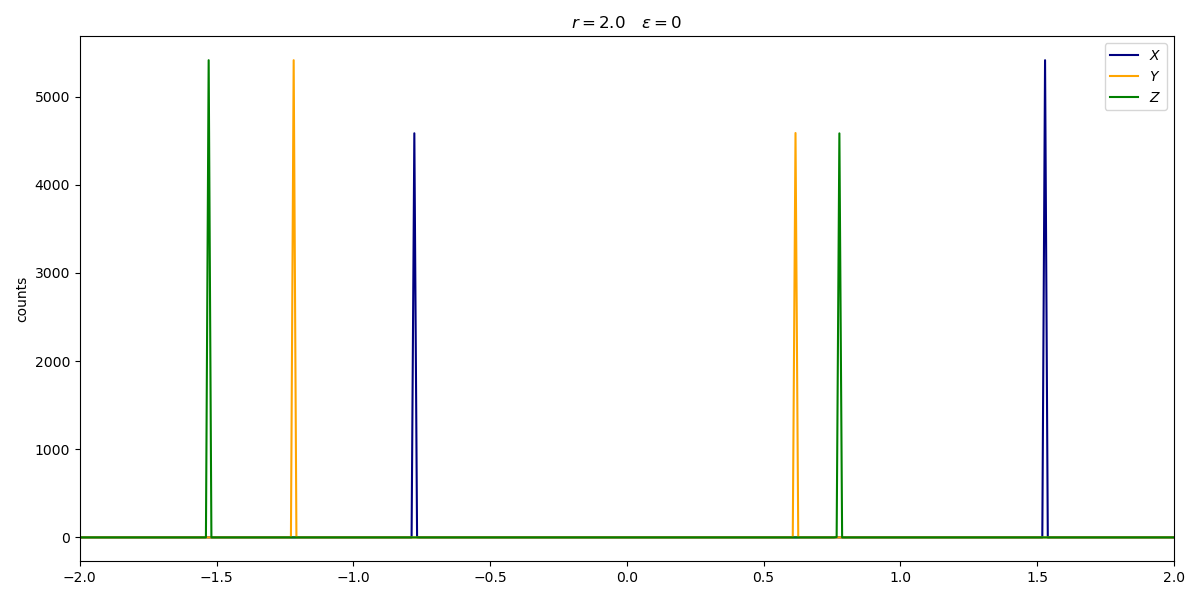
\includegraphics[width=\textwidth, height=0.52\textheight,keepaspectratio]{./figures_2/r2-noiseless-hist.png}
	\end{figure}
\end{frame}

\begin{frame}{Deterministic Bifurcation Diagram}
	\begin{figure}
	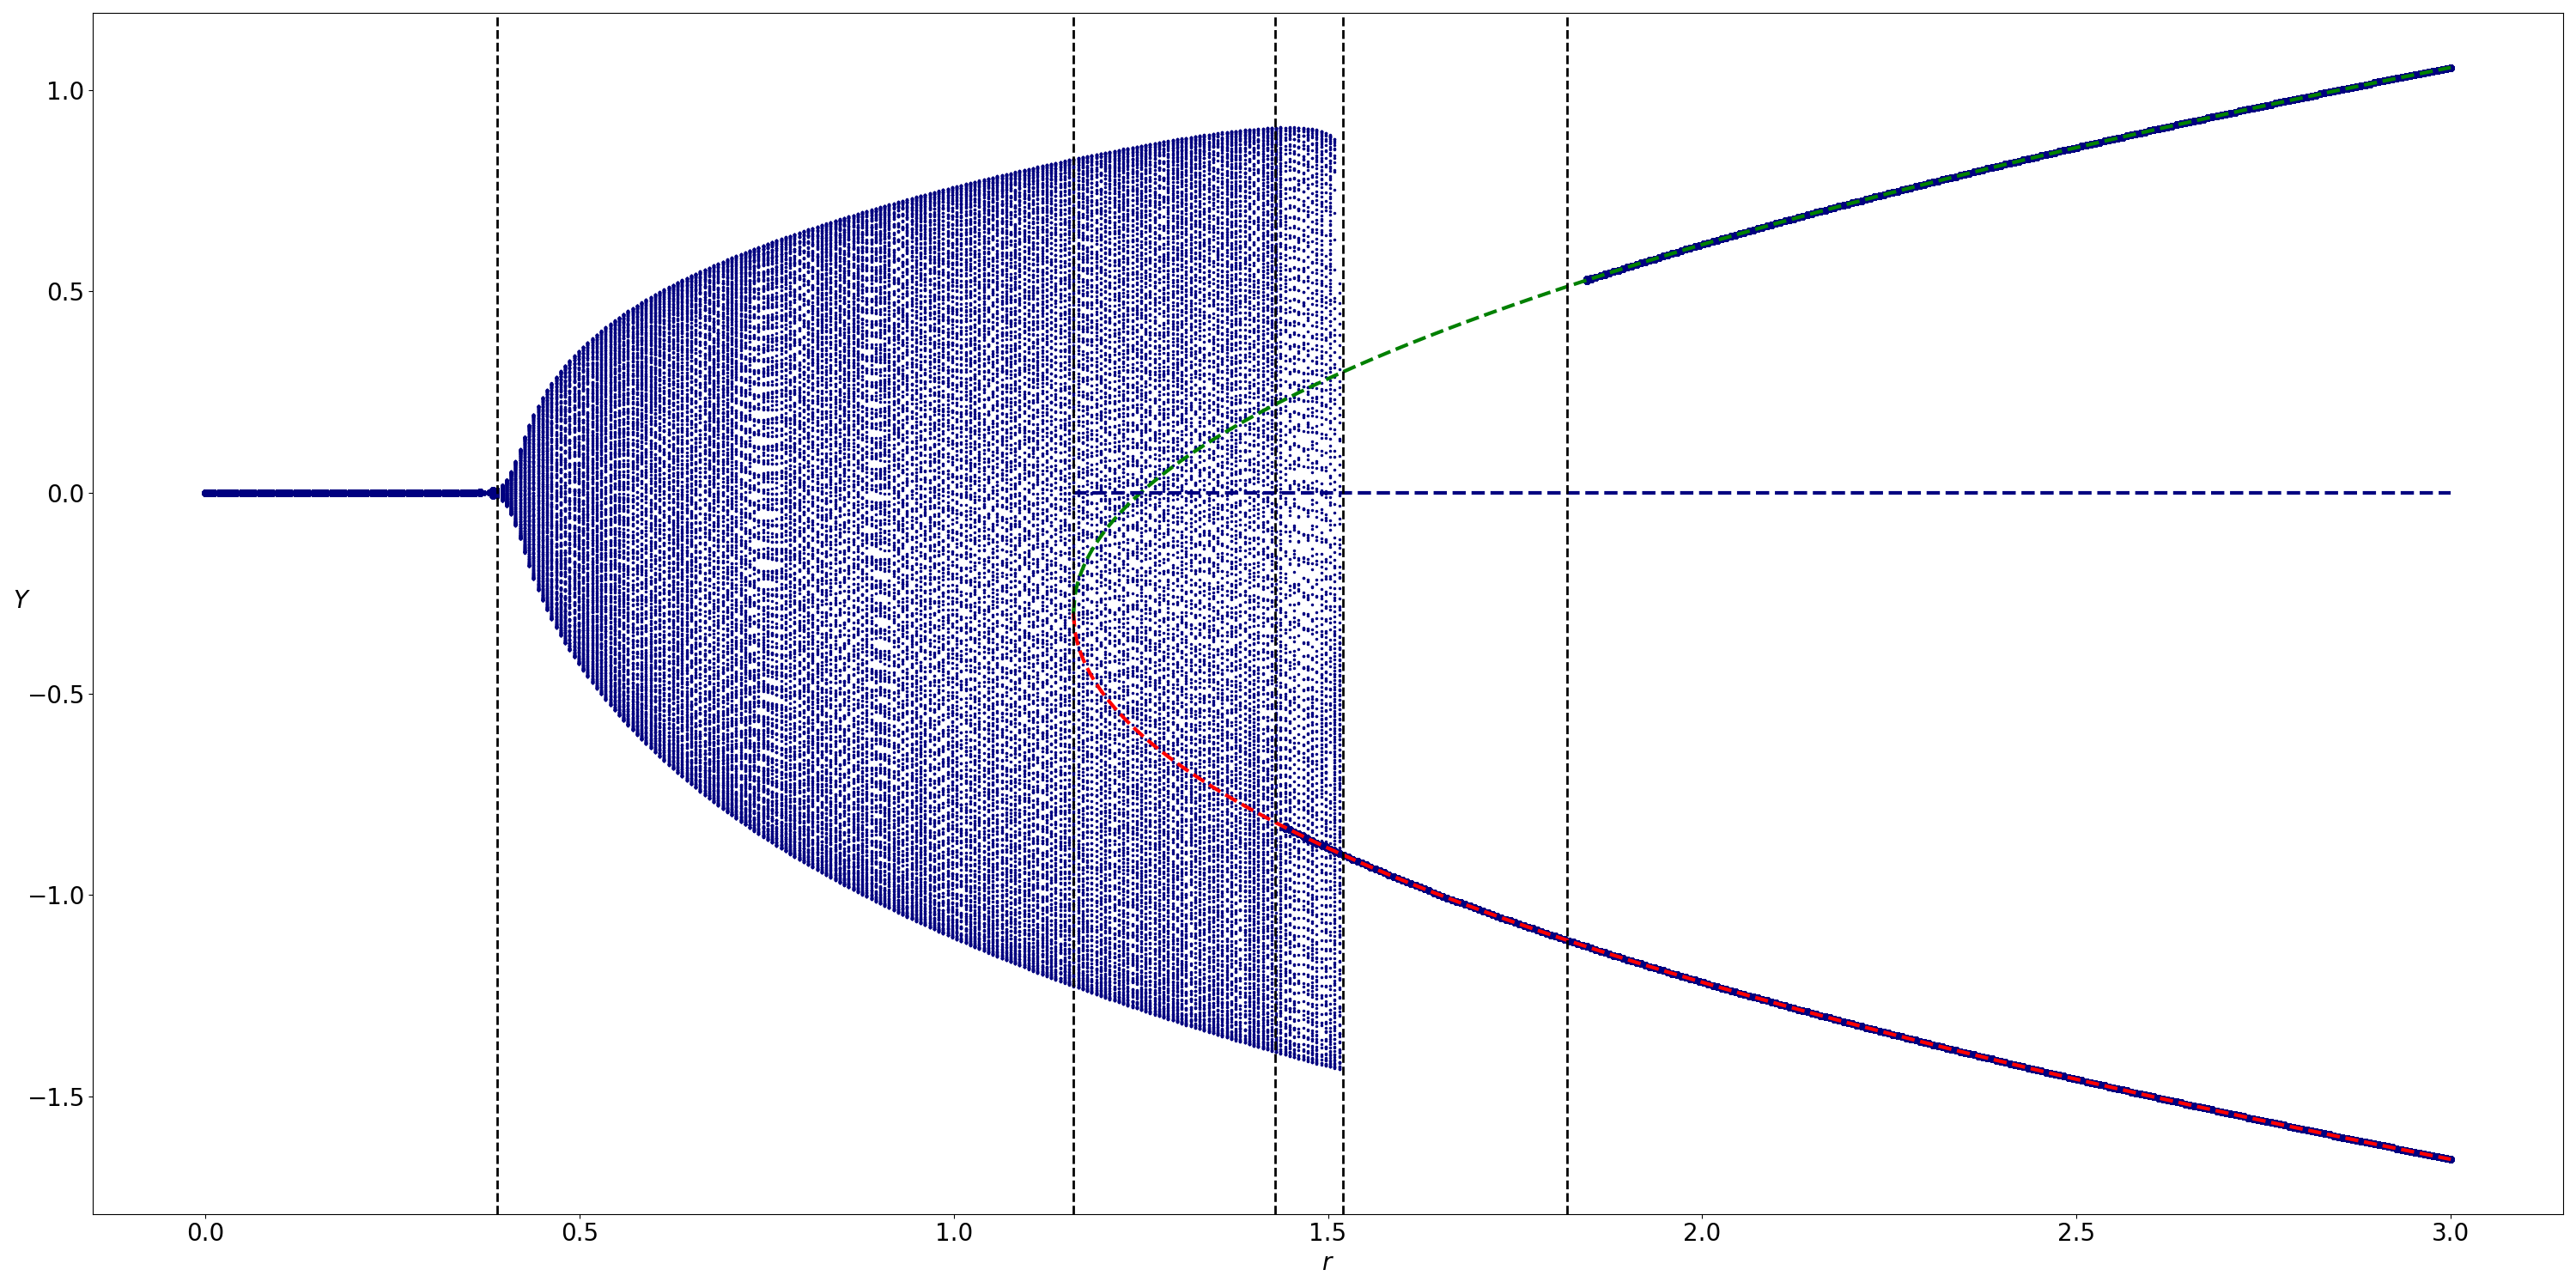
\includegraphics[width=\textwidth, height=\textheight,keepaspectratio]{figures_2/noiseless-phase-portrait.png}
	\end{figure}
	
	$E_0 = (0, 0, 0)$ is stable for $r < r_1 = 0.41704$. 
	At $r = r_1$, bifurcation with the birth of a stable limit cycle.
	This cycle loses its stability at $r_4 = 1.517$. 
	The equilibria $E_1, E_2$ appearing at $r = r_2 = 1.16$ are unstable at first. 
	The equilibrium $E_2$ becomes stable at $r_3 = 1.42271$, $E_1$ at $r_5 = 1.82025$.
\end{frame}

\begin{frame}{Deterministic Bifurcation Diagram}
	\begin{itemize}
		\item In the parametric region $0 < r < r_1$, the system is monostable with the trivial equilibrium $E_0$ as a single attractor. 
		\item In the zone $r_1 < r < r_3$ , the climate system is monostable with the stable limit cycle as a single attractor. 
		\item For $r_3 < r < r_4$, the system is bistable with two coexisting attractors, namely the equilibrium $E_2$ and the limit cycle. 
		\item For $r_4 < r < r_5$ , the deterministic system is monostable with the equilibrium $E_2$ representing a single attractor. 
		\item If $r > r_5$ , the system is bistable with two coexisting stable equilibria $E_1$ and $E_2$.
	\end{itemize}
\end{frame}



\section{The Stochastic Model}

\begin{frame}{The Stochastic Saltzman-Maasch model}
	Now a stochastic dynamics is introduced, in order to reveal new features 
	of noise-induced climate variability. 
	Introduce in the model a \textbf{multiplicative white gaussian 
	noise} term in the third equation.

	\[
		\begin{cases}
			\dot{X} = -X -Y -vZ \\ 
			\dot{Y} = -pZ + rY -sY^2 -Y^3 \\
			\dot{Z} = -q(X+Z) + \epsilon Z \xi(t)
		\end{cases}
	\]
	where $\xi(t)$ is the multiplicative white noise.

	It will be shown that the climate system can be highly noise-excitable and it 
	possesses large-amplitude fluctuations even in those regions where the 
	deterministic model does not contain any self-sustained oscillations.
\end{frame}

\begin{frame}{Noisy Trajectories: Noisy Phase Portraits}
	\begin{figure}
		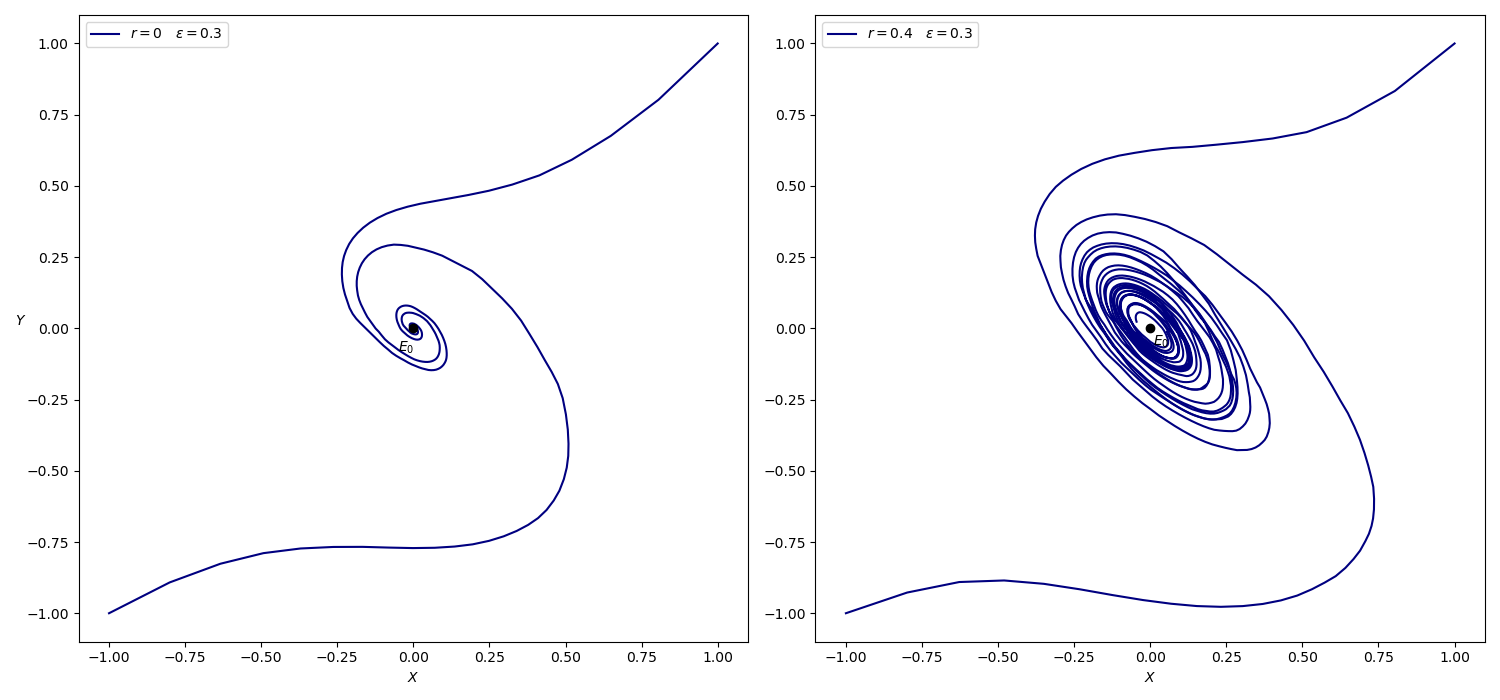
\includegraphics[width=0.82\textwidth, height=0.7\textheight,keepaspectratio]{./figures_2/r0-0.4-eps0.3-trajectories.png}
		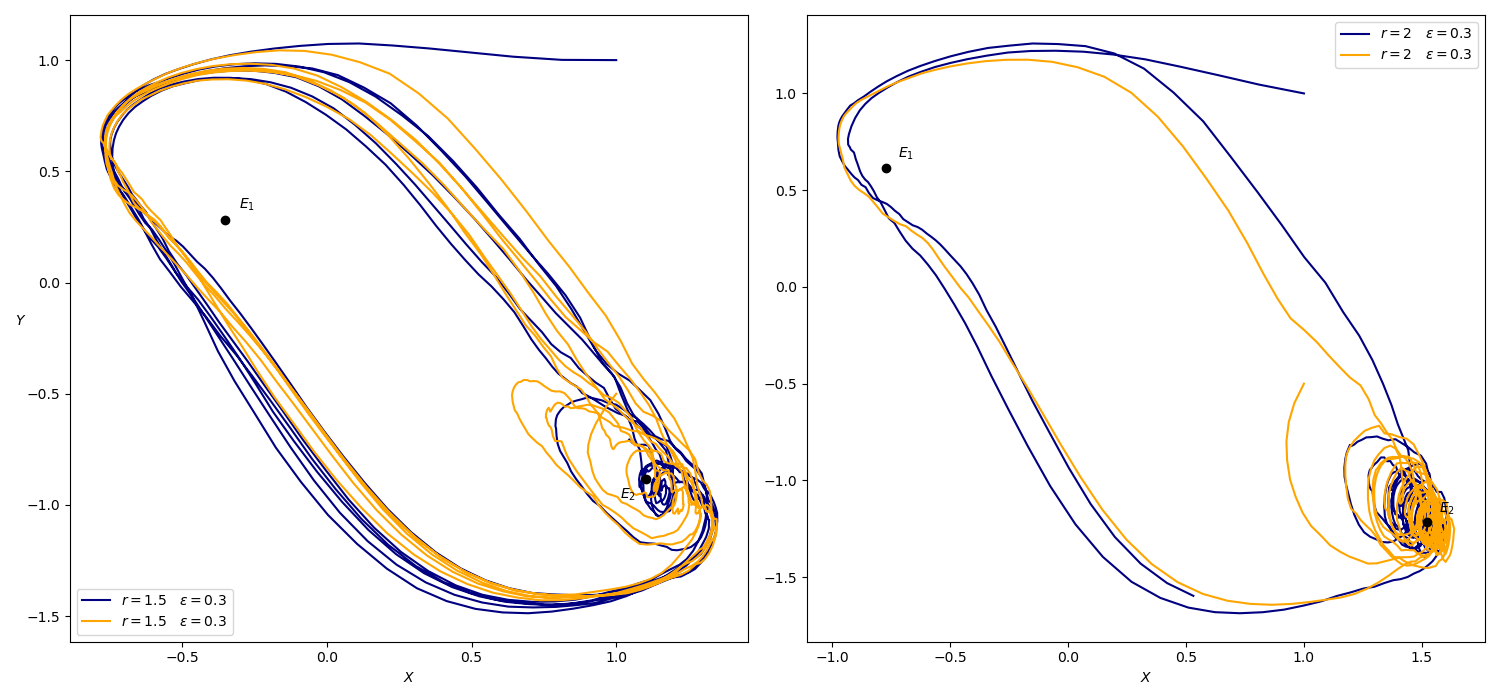
\includegraphics[width=0.82\textwidth, height=0.7\textheight,keepaspectratio]{./figures_2/r1.5-2-eps0.3-trajectories.png}
	\end{figure}
\end{frame}

%\begin{frame}{Attractors with White Noise}
%	\begin{figure}
%		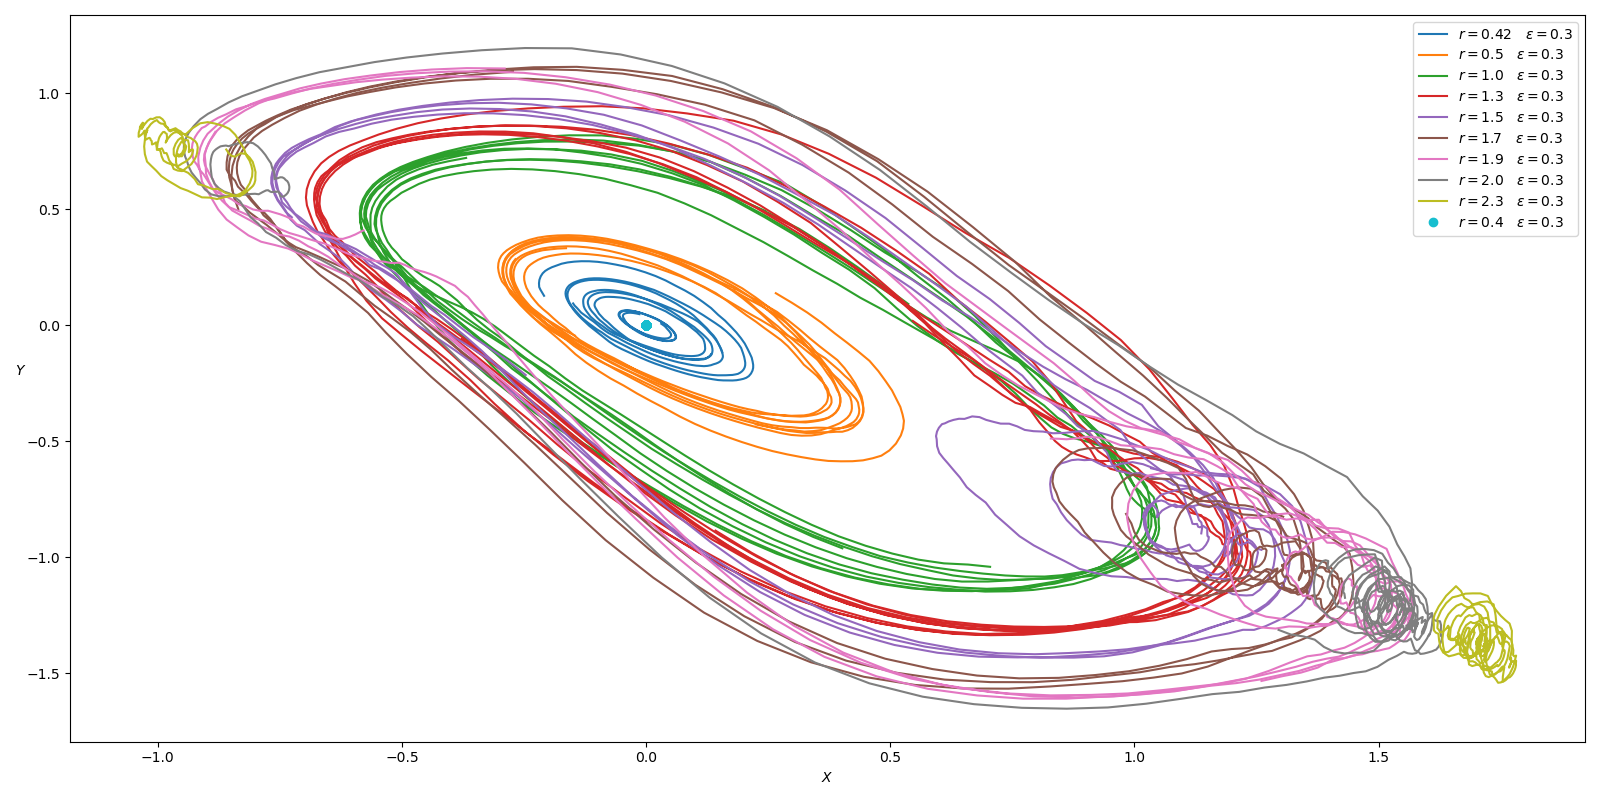
\includegraphics[width=\textwidth, height=\textheight,keepaspectratio]{./figures_2/eps0.3-attractors.png}
%	\end{figure}
%
%	Some comments....
%\end{frame}

\begin{frame}{Time Behavior and Histograms}
	\begin{figure}
		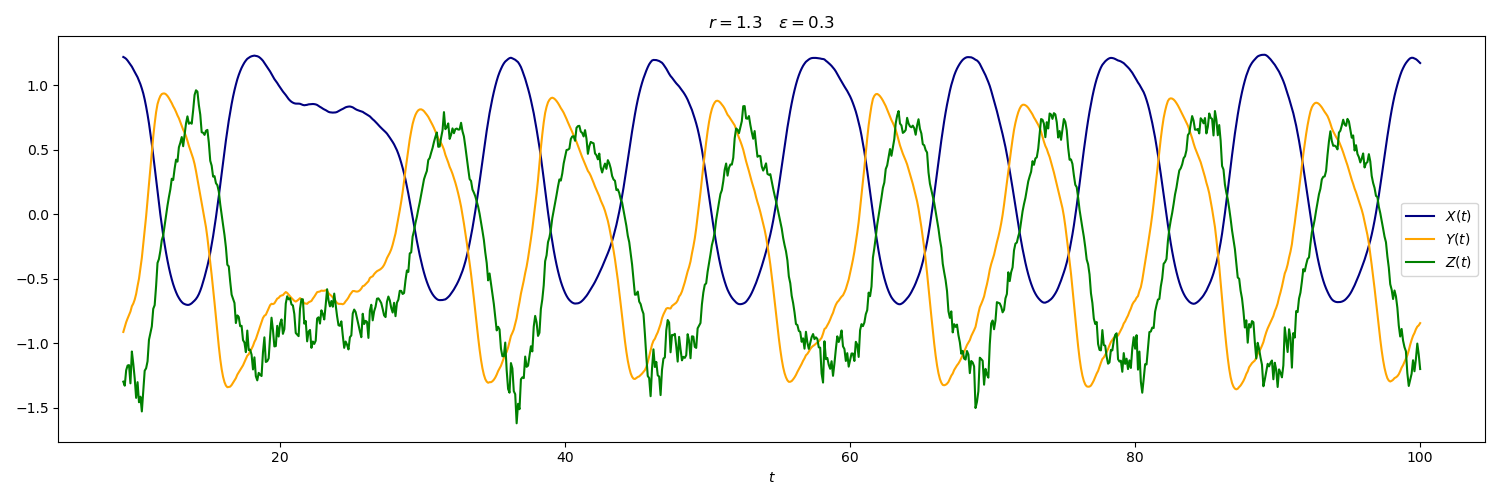
\includegraphics[width=\textwidth, height=0.52\textheight,keepaspectratio]{./figures_2/r1.3-eps0.3-time-trajectories.png}
		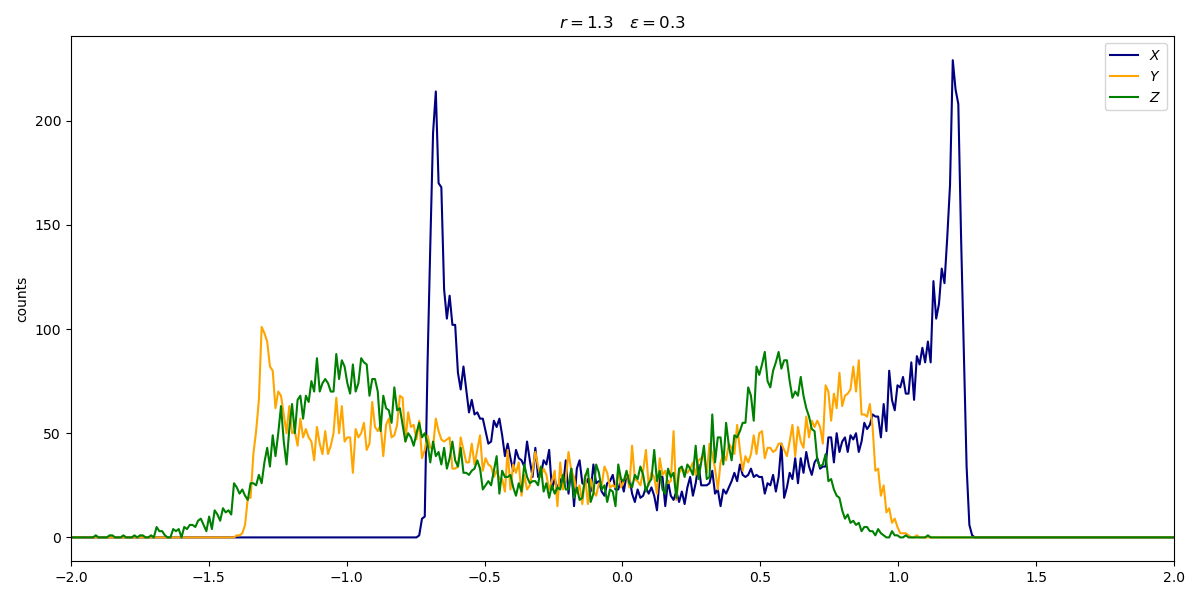
\includegraphics[width=\textwidth, height=0.52\textheight,keepaspectratio]{./figures_2/r1.3-eps0.3-hist.png}
	\end{figure}
\end{frame}

\begin{frame}{Time Behavior and Histograms}
	\begin{figure}
		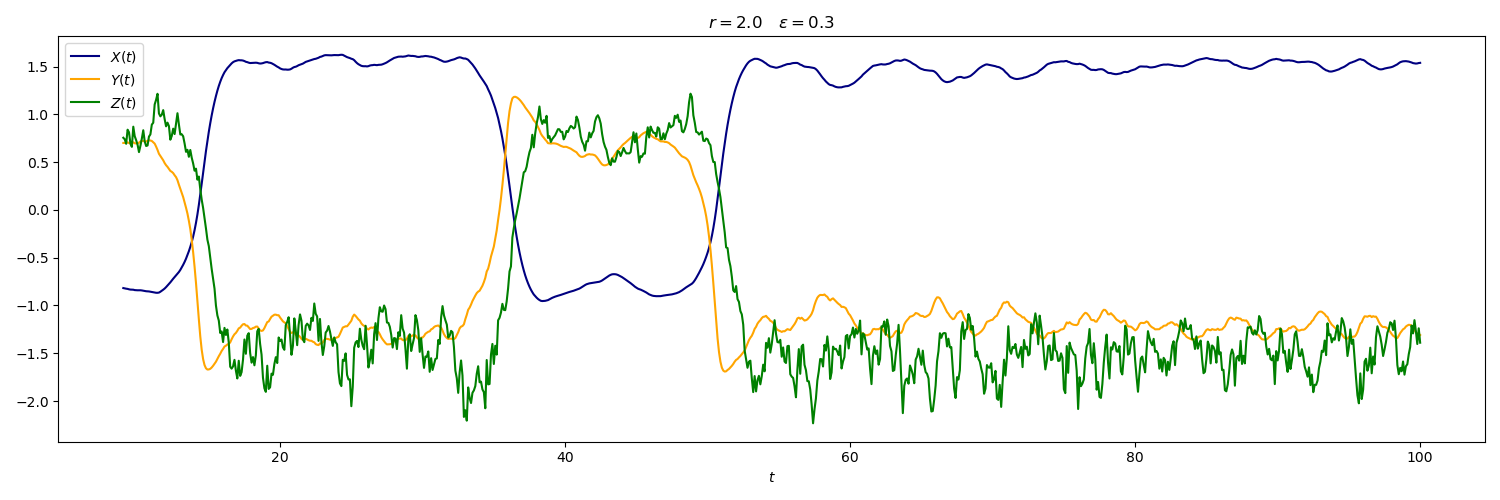
\includegraphics[width=\textwidth, height=0.52\textheight,keepaspectratio]{./figures_2/r2-eps0.3-time-trajectories.png}
		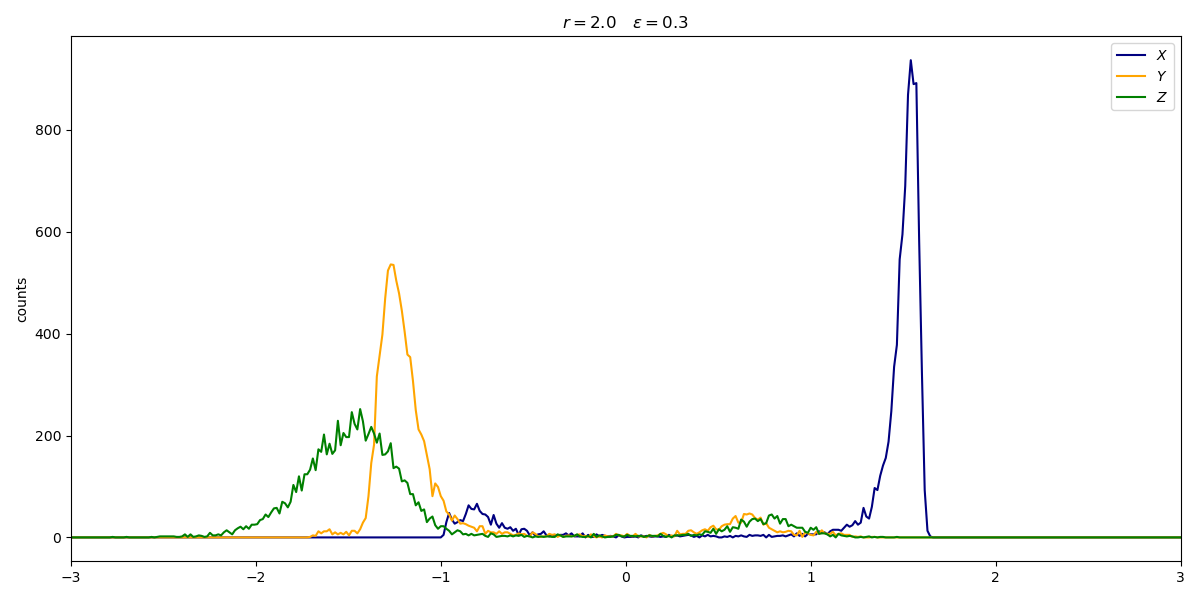
\includegraphics[width=\textwidth, height=0.52\textheight,keepaspectratio]{./figures_2/r2-eps0.3-hist.png}
	\end{figure}
\end{frame}

\begin{frame}{Bifurcation Diagram with Noise}
	How the Phase Portrait has changed under the effect of noise: presence of noise-induced phenomena of transition.
	\begin{figure}
	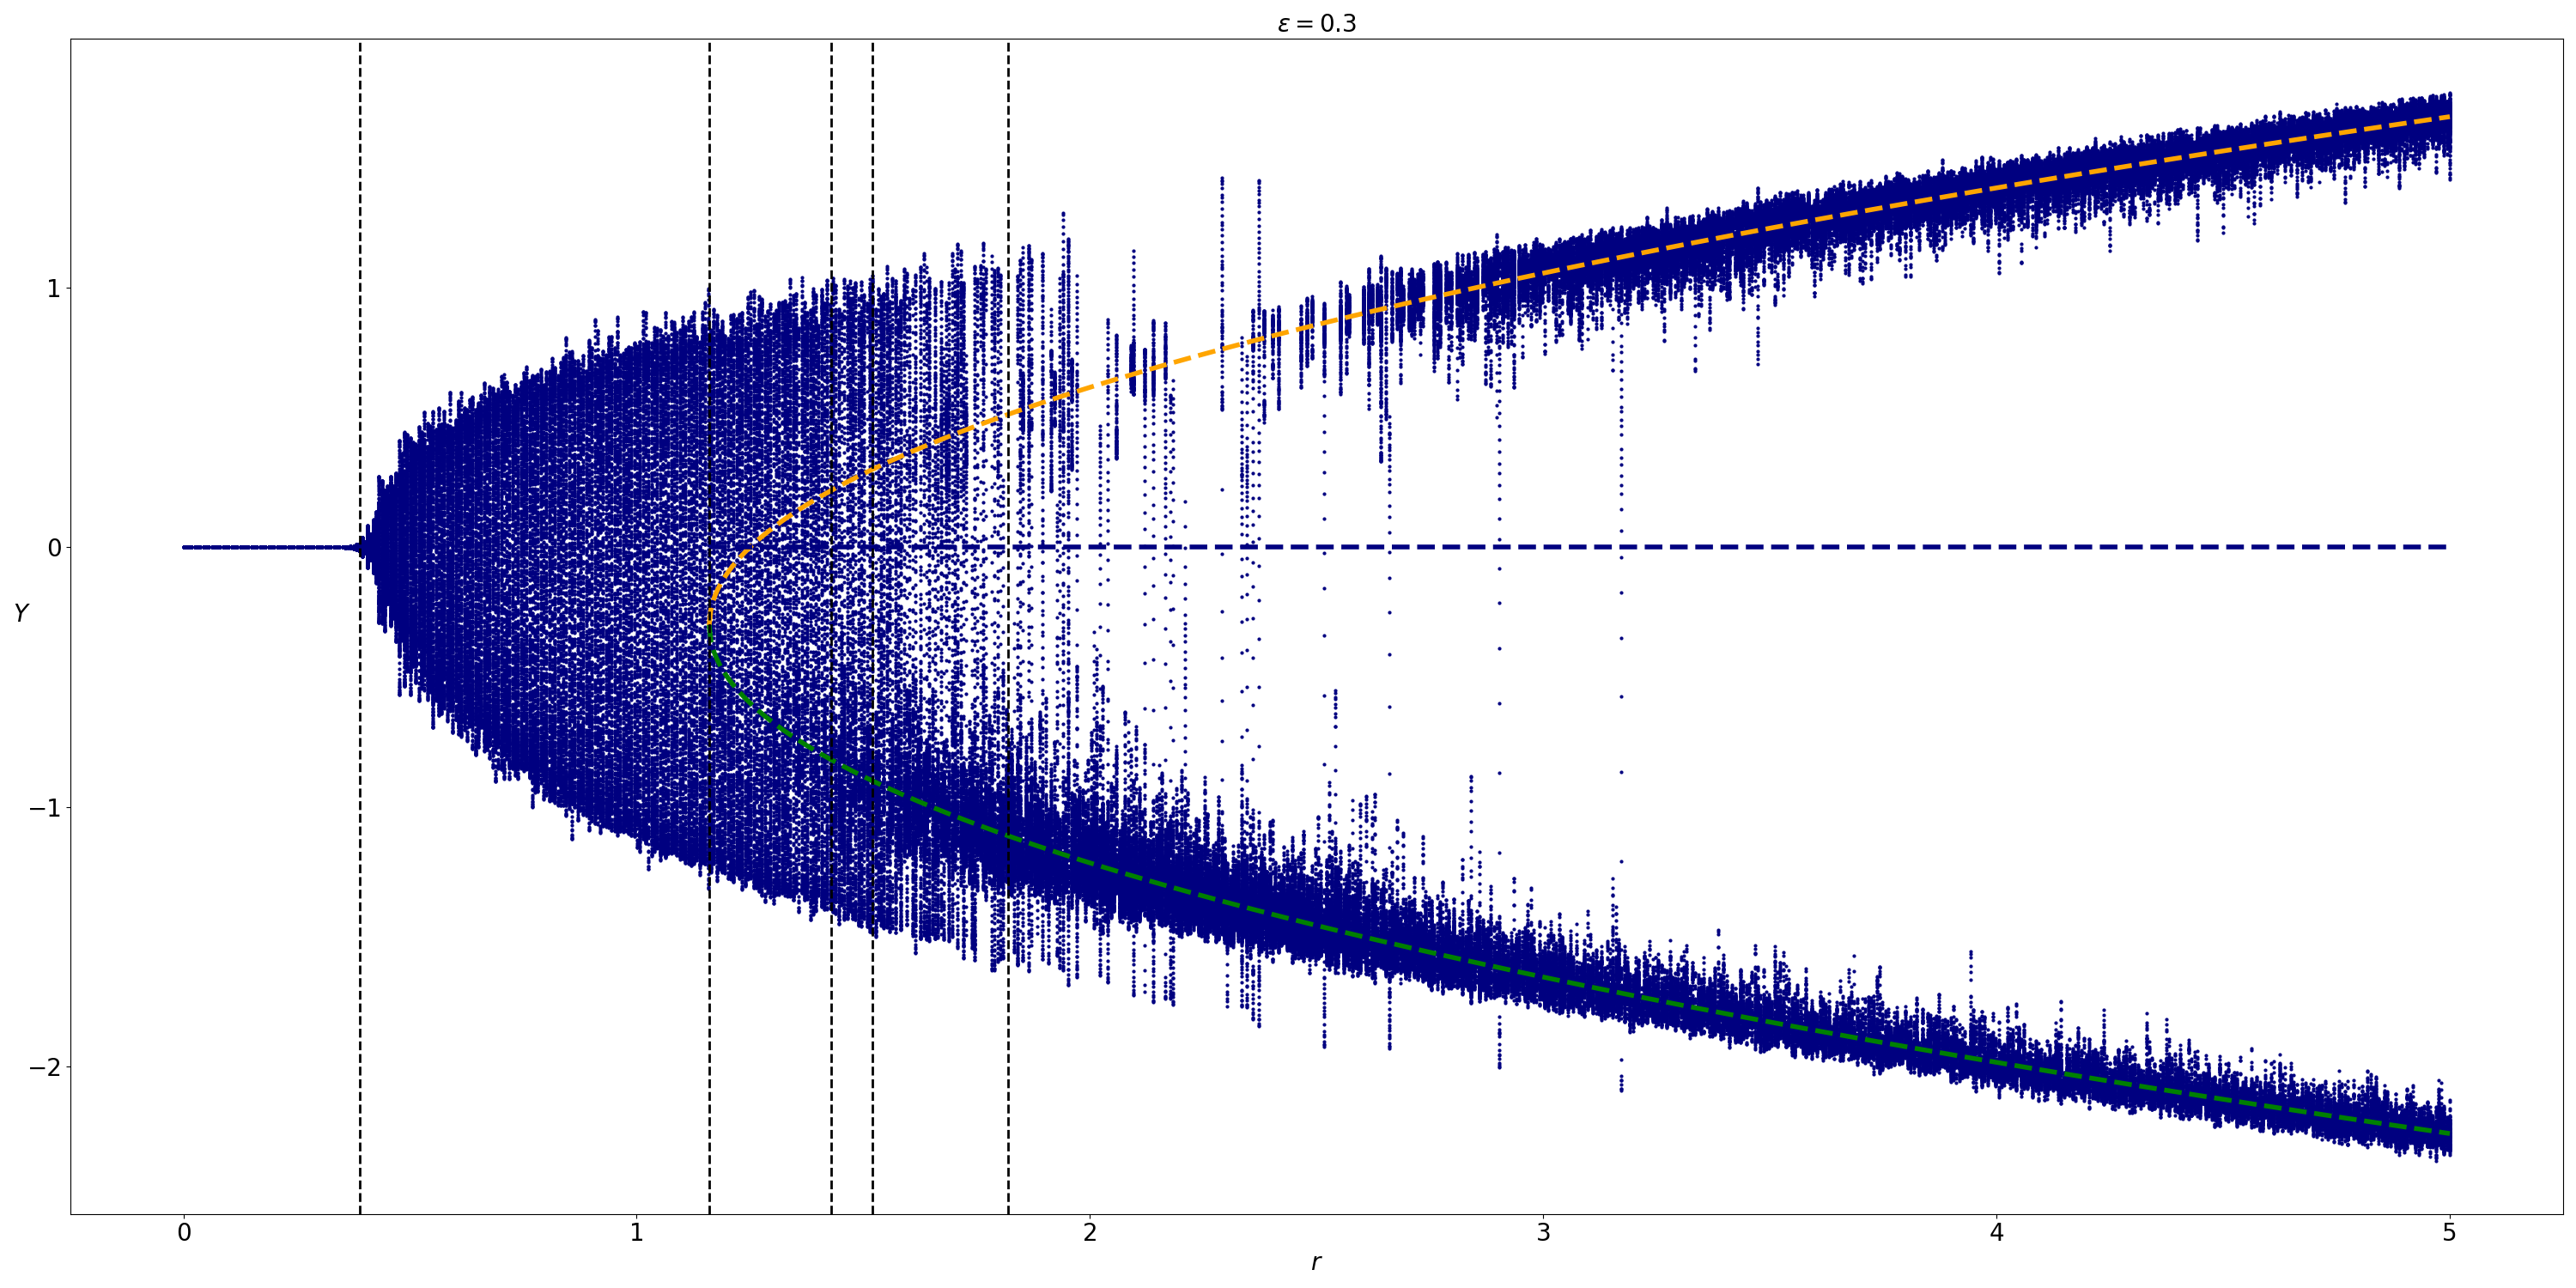
\includegraphics[width=\textwidth, height=\textheight,keepaspectratio]{figures_2/eps0.3-phase-portrait.png}
	\end{figure}
\end{frame}

\begin{frame}{NITs}
	\begin{figure}
		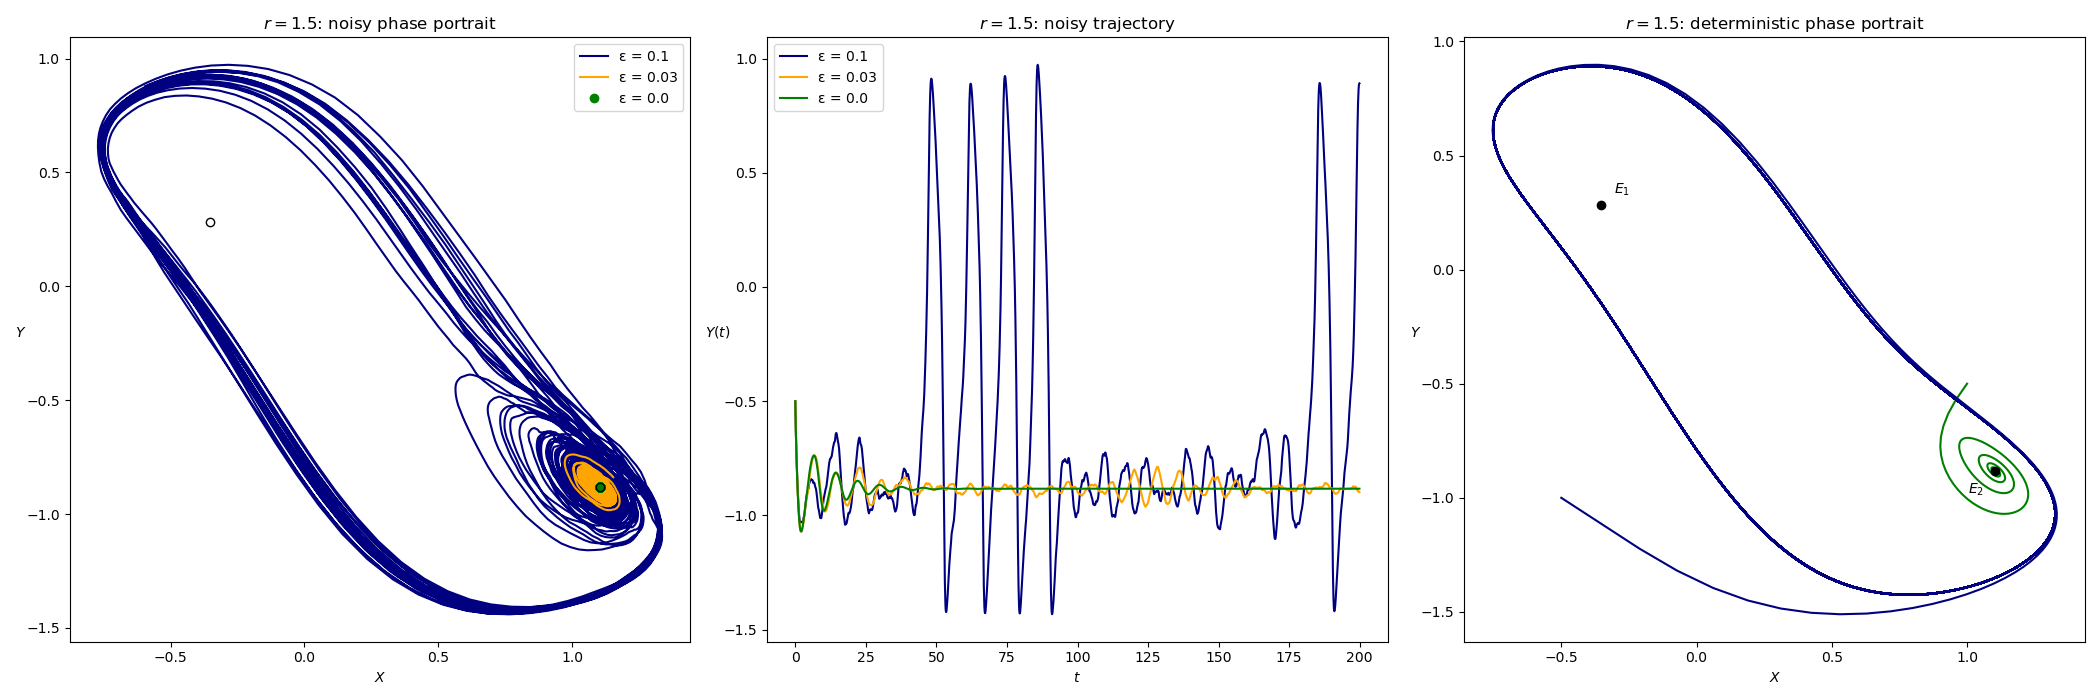
\includegraphics[width=\textwidth, height=\textheight,keepaspectratio]{./figures_2/NIT-r1.5.png}
	\end{figure}

	\begin{itemize}
		\item $r = 1.5$: bistability region $r_3 < r < r_4$.
		\item For weak noise, $\epsilon=0.03$, the solutions exhibit small
		amplitude stochastically-induced oscillations (SASIO) near $E_2$
		\item With increasing noise, the system starts to demonstrate large amplitude 
		stochastically-induced oscillations (LASIO)
		\item This change is due to noise-induced 
		transitions between the basins of attraction of the equilibrium 
		$E_2$ and the periodic cycle
	\end{itemize}
\end{frame}

\begin{frame}{NITs}
	\begin{figure}
		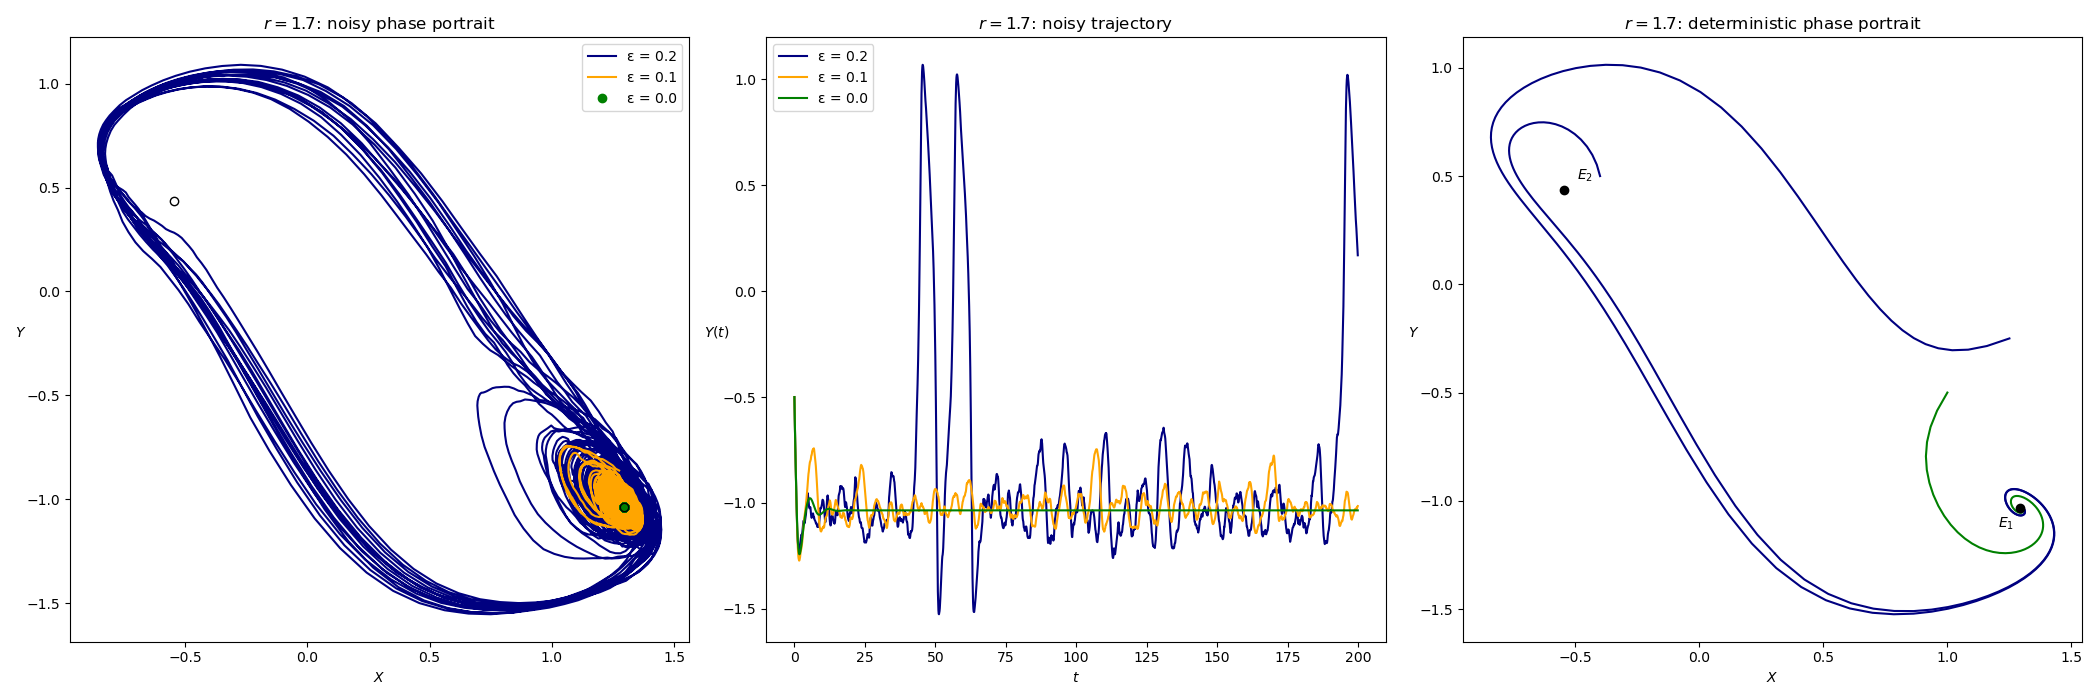
\includegraphics[width=\textwidth, height=0.52\textheight,keepaspectratio]{./figures_2/NIT-r1.7.png}
	\end{figure}

	\begin{itemize}
		\item Monostability region with $r=1.7$: $E_2$ as single attractor and no stable cycles
		\item For small deviations of initial states (subthreshold zone), the trajectories 
		tend to $E_2$. For larger deviations (superthreshold zone), the 
		trajectory exhibits a large-amplitude loop
		\item For $\epsilon = 0.1$, SASIO is observed near $E_2$, while for 
		$\epsilon = 0.2$, a complex regime with alternating SASIO and LASIO is evident
	\end{itemize}
\end{frame}

\begin{frame}{NITs}
	\begin{figure}
		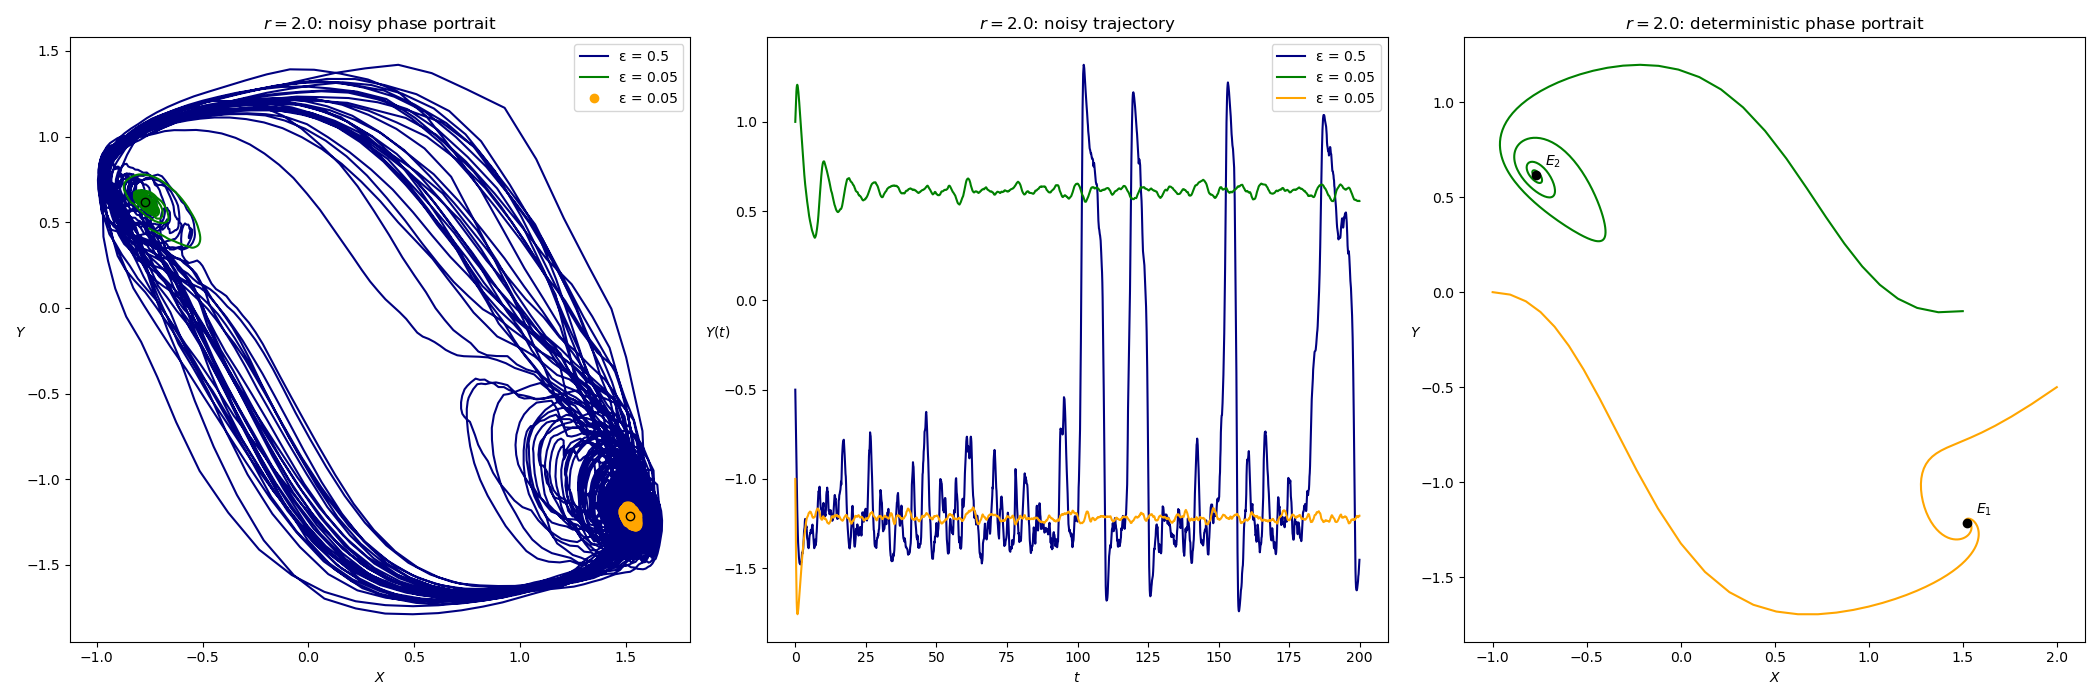
\includegraphics[width=\textwidth, height=0.52\textheight,keepaspectratio]{./figures_2/NIT-r2.png}
	\end{figure}

	\begin{itemize}
		\item For $r = 1.9$, the deterministic system 
		has two stable equilibria, $E_1$ (warm climate state, in orange) and $E_2$ (cold state, in green)
		\item For $\epsilon = 0.05$, the solutions starting near $E_1$ and $E_2$ 
		are concentrated near their corresponding equilibria (subthreshold)
		\item With increasing noise, mutual transitions between 
		the basins of attraction of these equilibria are revealed with complex 
		oscillatory regime with alternating SASIO and LASIO
	\end{itemize}
\end{frame}

\begin{frame}{NITs}
	\begin{figure}
	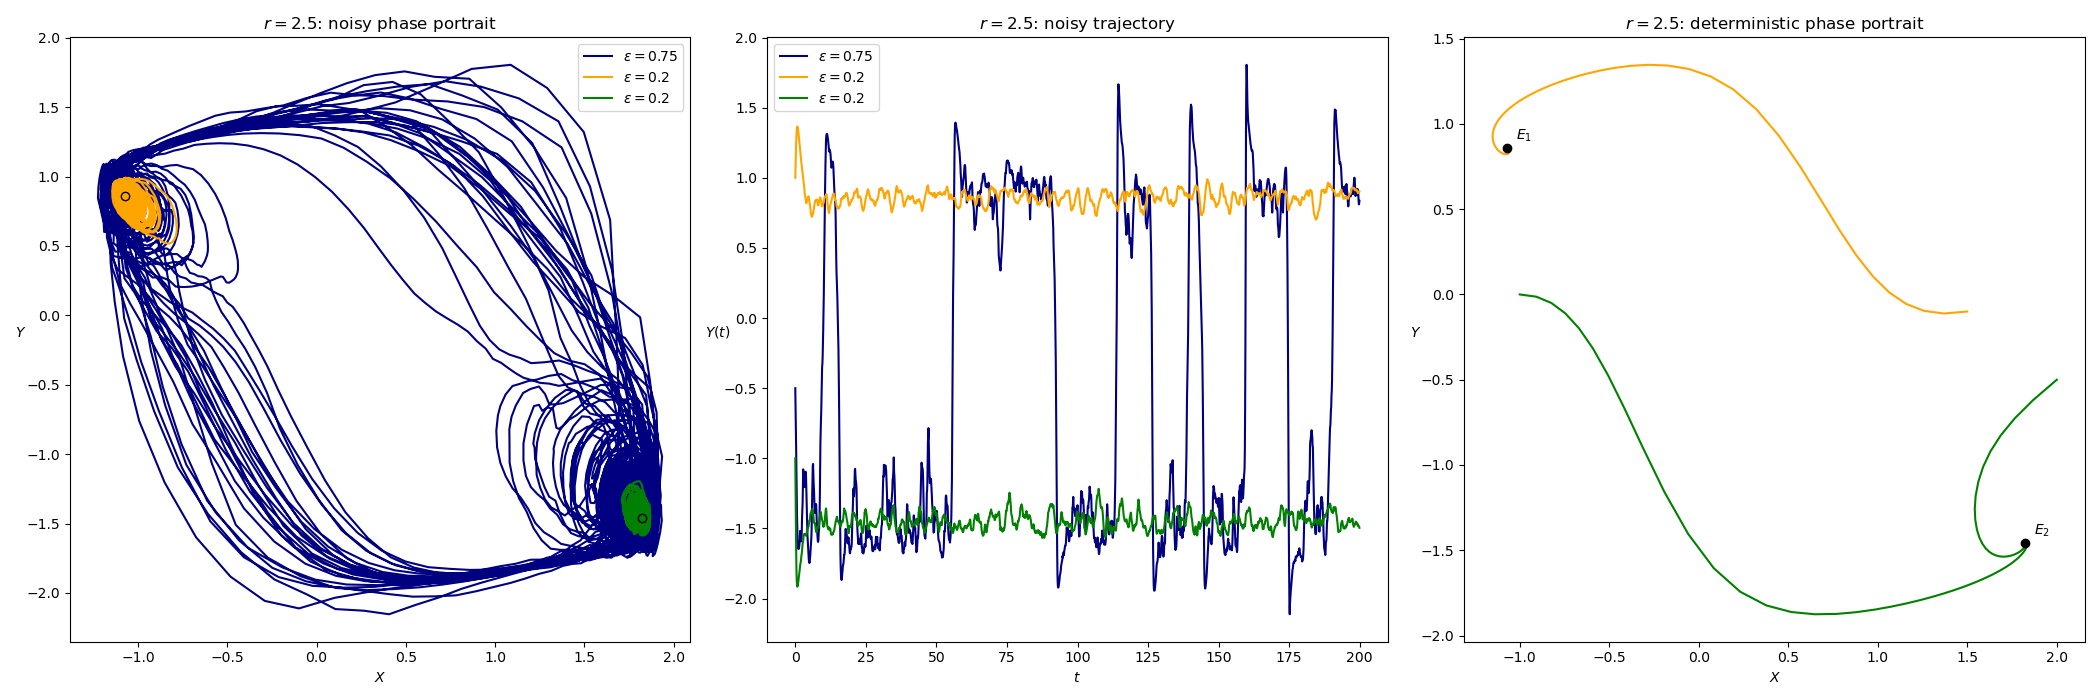
\includegraphics[width=\textwidth, height=\textheight,keepaspectratio]{figures_2/NIT-r2.5.png}
	\end{figure}
	
	\begin{itemize}
		\item For $\epsilon = 0.2$, solutions starting near $E_1$, result in 
		small-amplitude oscillations
		\item As noise increases, trajectories fall into the superthreshold zone, 
		then to the subthreshold zone of equilibrium $E_2$ exhibiting SASIO
		\item With further noise increase, trajectories fall into the superthreshold 
		zone of equilibrium $E_2$, generating large-amplitude oscillations around both 
		$E_1$ and $E_2$
	\end{itemize}
\end{frame}

\begin{frame}{NITs}
	\begin{figure}
	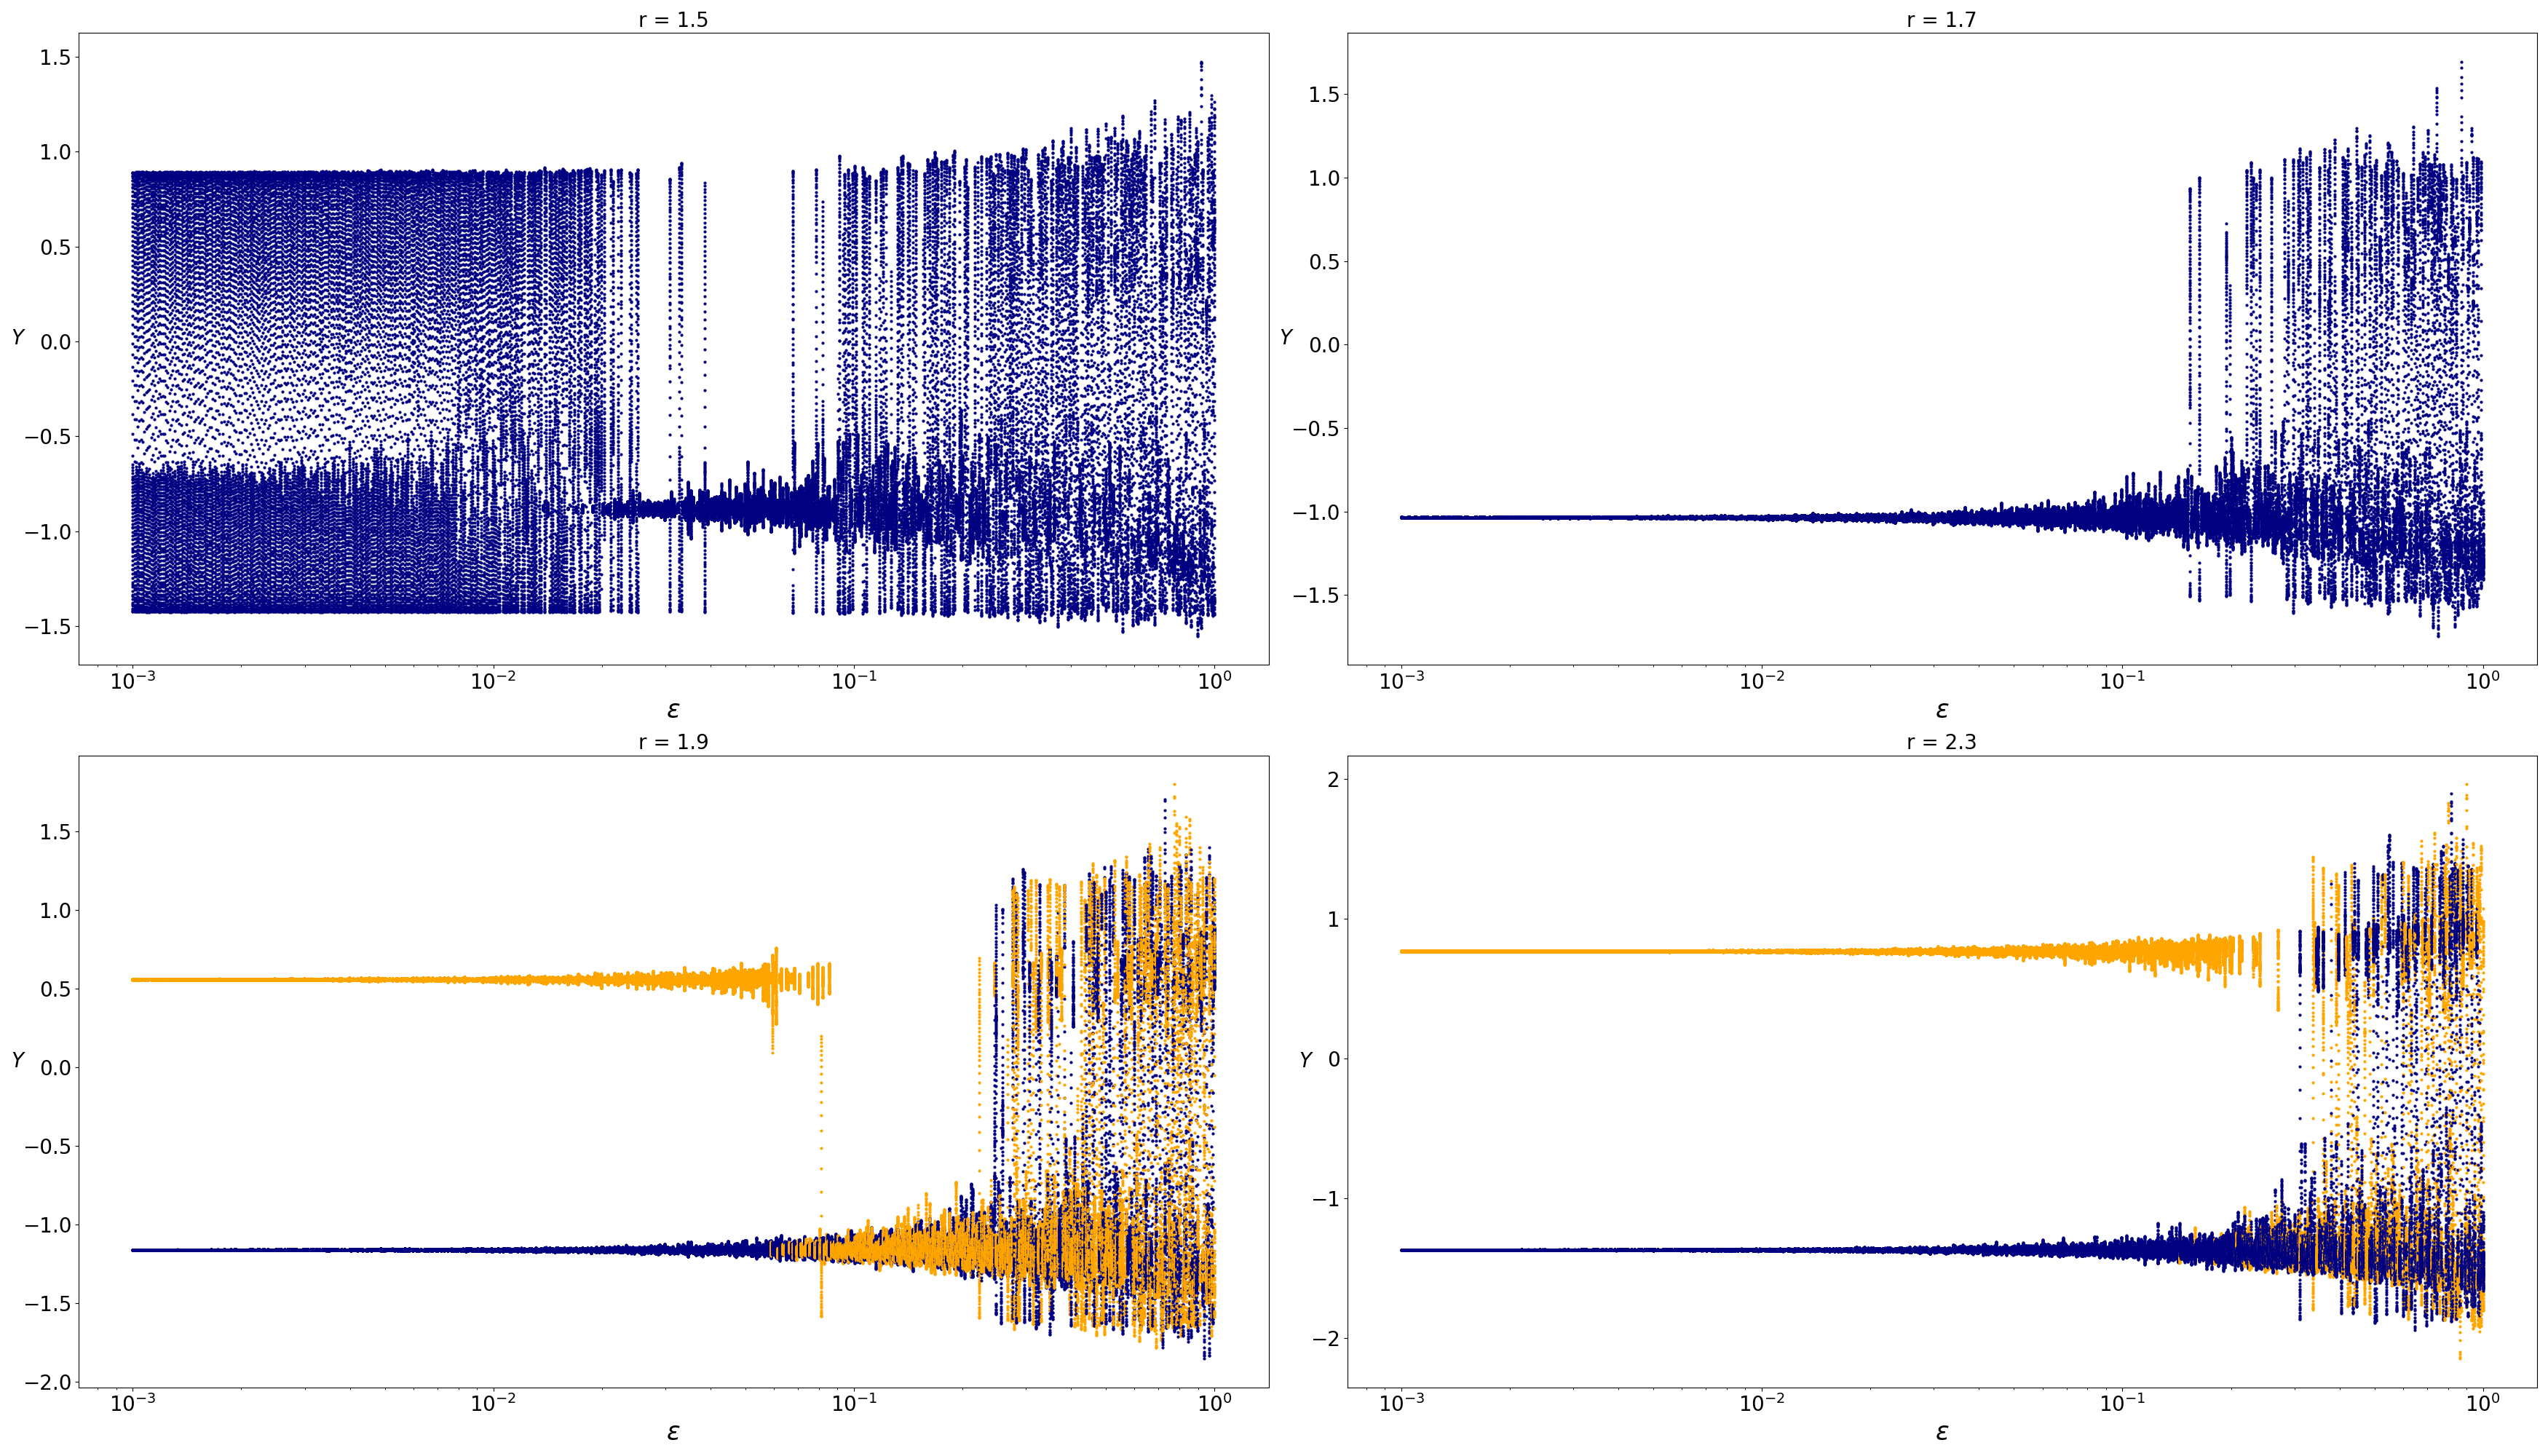
\includegraphics[width=\textwidth, height=\textheight,keepaspectratio]{figures_2/NITvseps1.png}
	\end{figure}
\end{frame}

\begin{frame}{NITs}
	Interesting multiphase process of stochastic noise-induced transformations
	in the bistability zone $r > r_5\approx 1.82$
	\begin{itemize}
		\item If a trajectory begins near 
		$E_2$ (in blue), increasing noise reveals only two phases: small 
		amplitude stochastic oscillations (SASIO) near $E_1$ and large amplitude 
		stochastic oscillations (LASIO) between $E_1$ and $E_2$
		\item If the trajectory starts from $E_1$ (in orange), three phases are 
		observed: SASIO near $E_1$, a transition to SASIO near $E_2$, and LASIO 
		between $E_1$ and $E_2$. This reveals a sharp transition from warm to cold 
		climate state
	\end{itemize}
\end{frame}


\section{Improved Model}

\begin{frame}{Improved Saltzman-Maasch model}
	\begin{enumerate}
		\item Generalize the deterministic part of the model, adding nonlinearities 
		and coupling terms
		\item Generalize the multiplicative stochastic term: use a more sophisticated 
		noise term, such as an Orstein-Uhlenbeck process $\eta(t)$, and incorporating a 
		different dependency on the variables
		\item Including external stochastic forcing terms
	\end{enumerate}
	\[
		\begin{cases}
			\dot{X} = -a(X+Y) -vZ + \omega_X \xi(t) \\ 
			\dot{Y} = -pZ + rY -sY^2 -Y^3 +bYZ +cZY^2 + \omega_Y \xi(t)\\
			\dot{Z} = -q(X+Z) + \epsilon Z (1 + dX) \eta(t)
		\end{cases}
	\]
	where:
	\begin{itemize}
		\item $a, b, c, d \geq 0$
		\item $\xi(t)$ is a white noise term
		\item $\eta(t)$ can be a white noise term, or an Ornstein-Uhlenbeck process
	\end{itemize}
\end{frame}

\begin{frame}{Equilibrium Points}
	In addition to the equilibrium $E_0=(0,0,0)$, the new model presents equilibrium points corresponding to the values of $Y$:
	\[
	Y_{1, 2} = \frac{\frac{ba}{a-v}-s \pm \sqrt{\left(\frac{ba}{a-v}-s\right)^2-4\left(\frac{ca}{a-v}-1\right)\left(r-\frac{pa}{a-v}\right)}} {2\left(1-\frac{ca}{a-v}\right)}
	\]
	
	which leads to the non-trivial equilibrium points expression:
	\[
	E_{1,2} = \left(-\frac{aY_{1,2}}{a-v}, \ Y_{1,2} \ , \ \frac{aY_{1,2}}{a-v}\right)
	\]

	For $b=c=0$ and $a=1$, we obtain the previous deterministic model.
\end{frame}

\begin{frame}{Effects of the parameters $b$ and $c$}
	\begin{figure}
		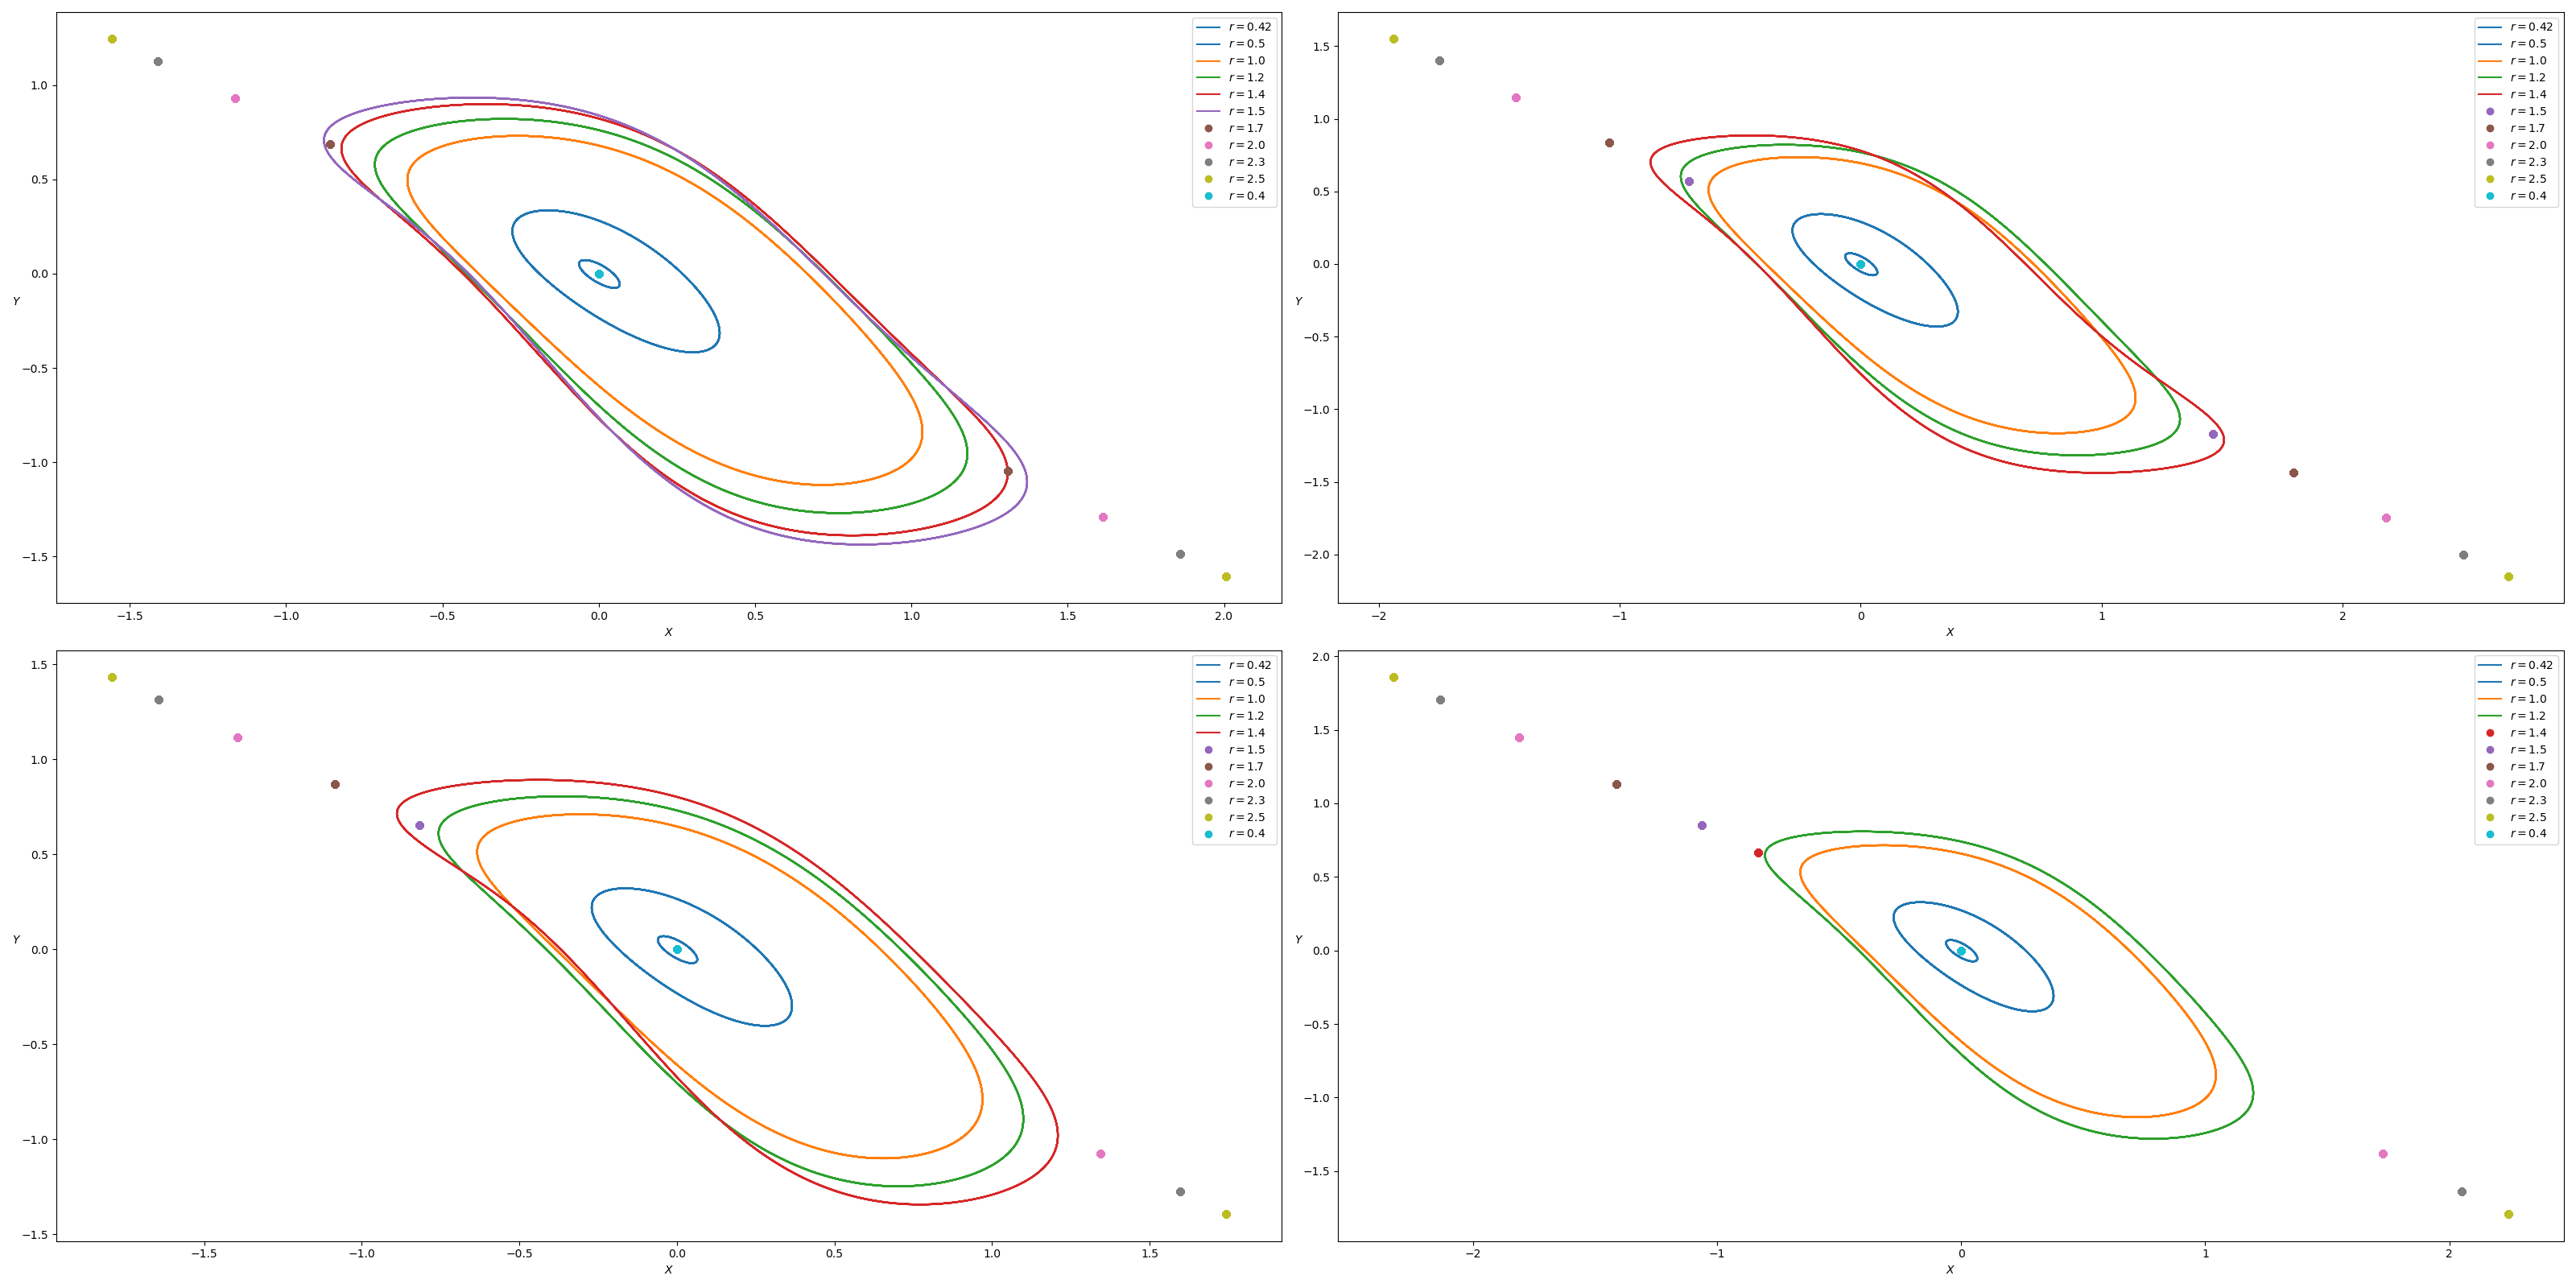
\includegraphics[width=\textwidth, height=\textheight,keepaspectratio]{figures_2/adv-attractors-b-c-2.png}
	\end{figure}
\end{frame}

\begin{frame}{Effects of the parameter $a$}
	\begin{figure}
		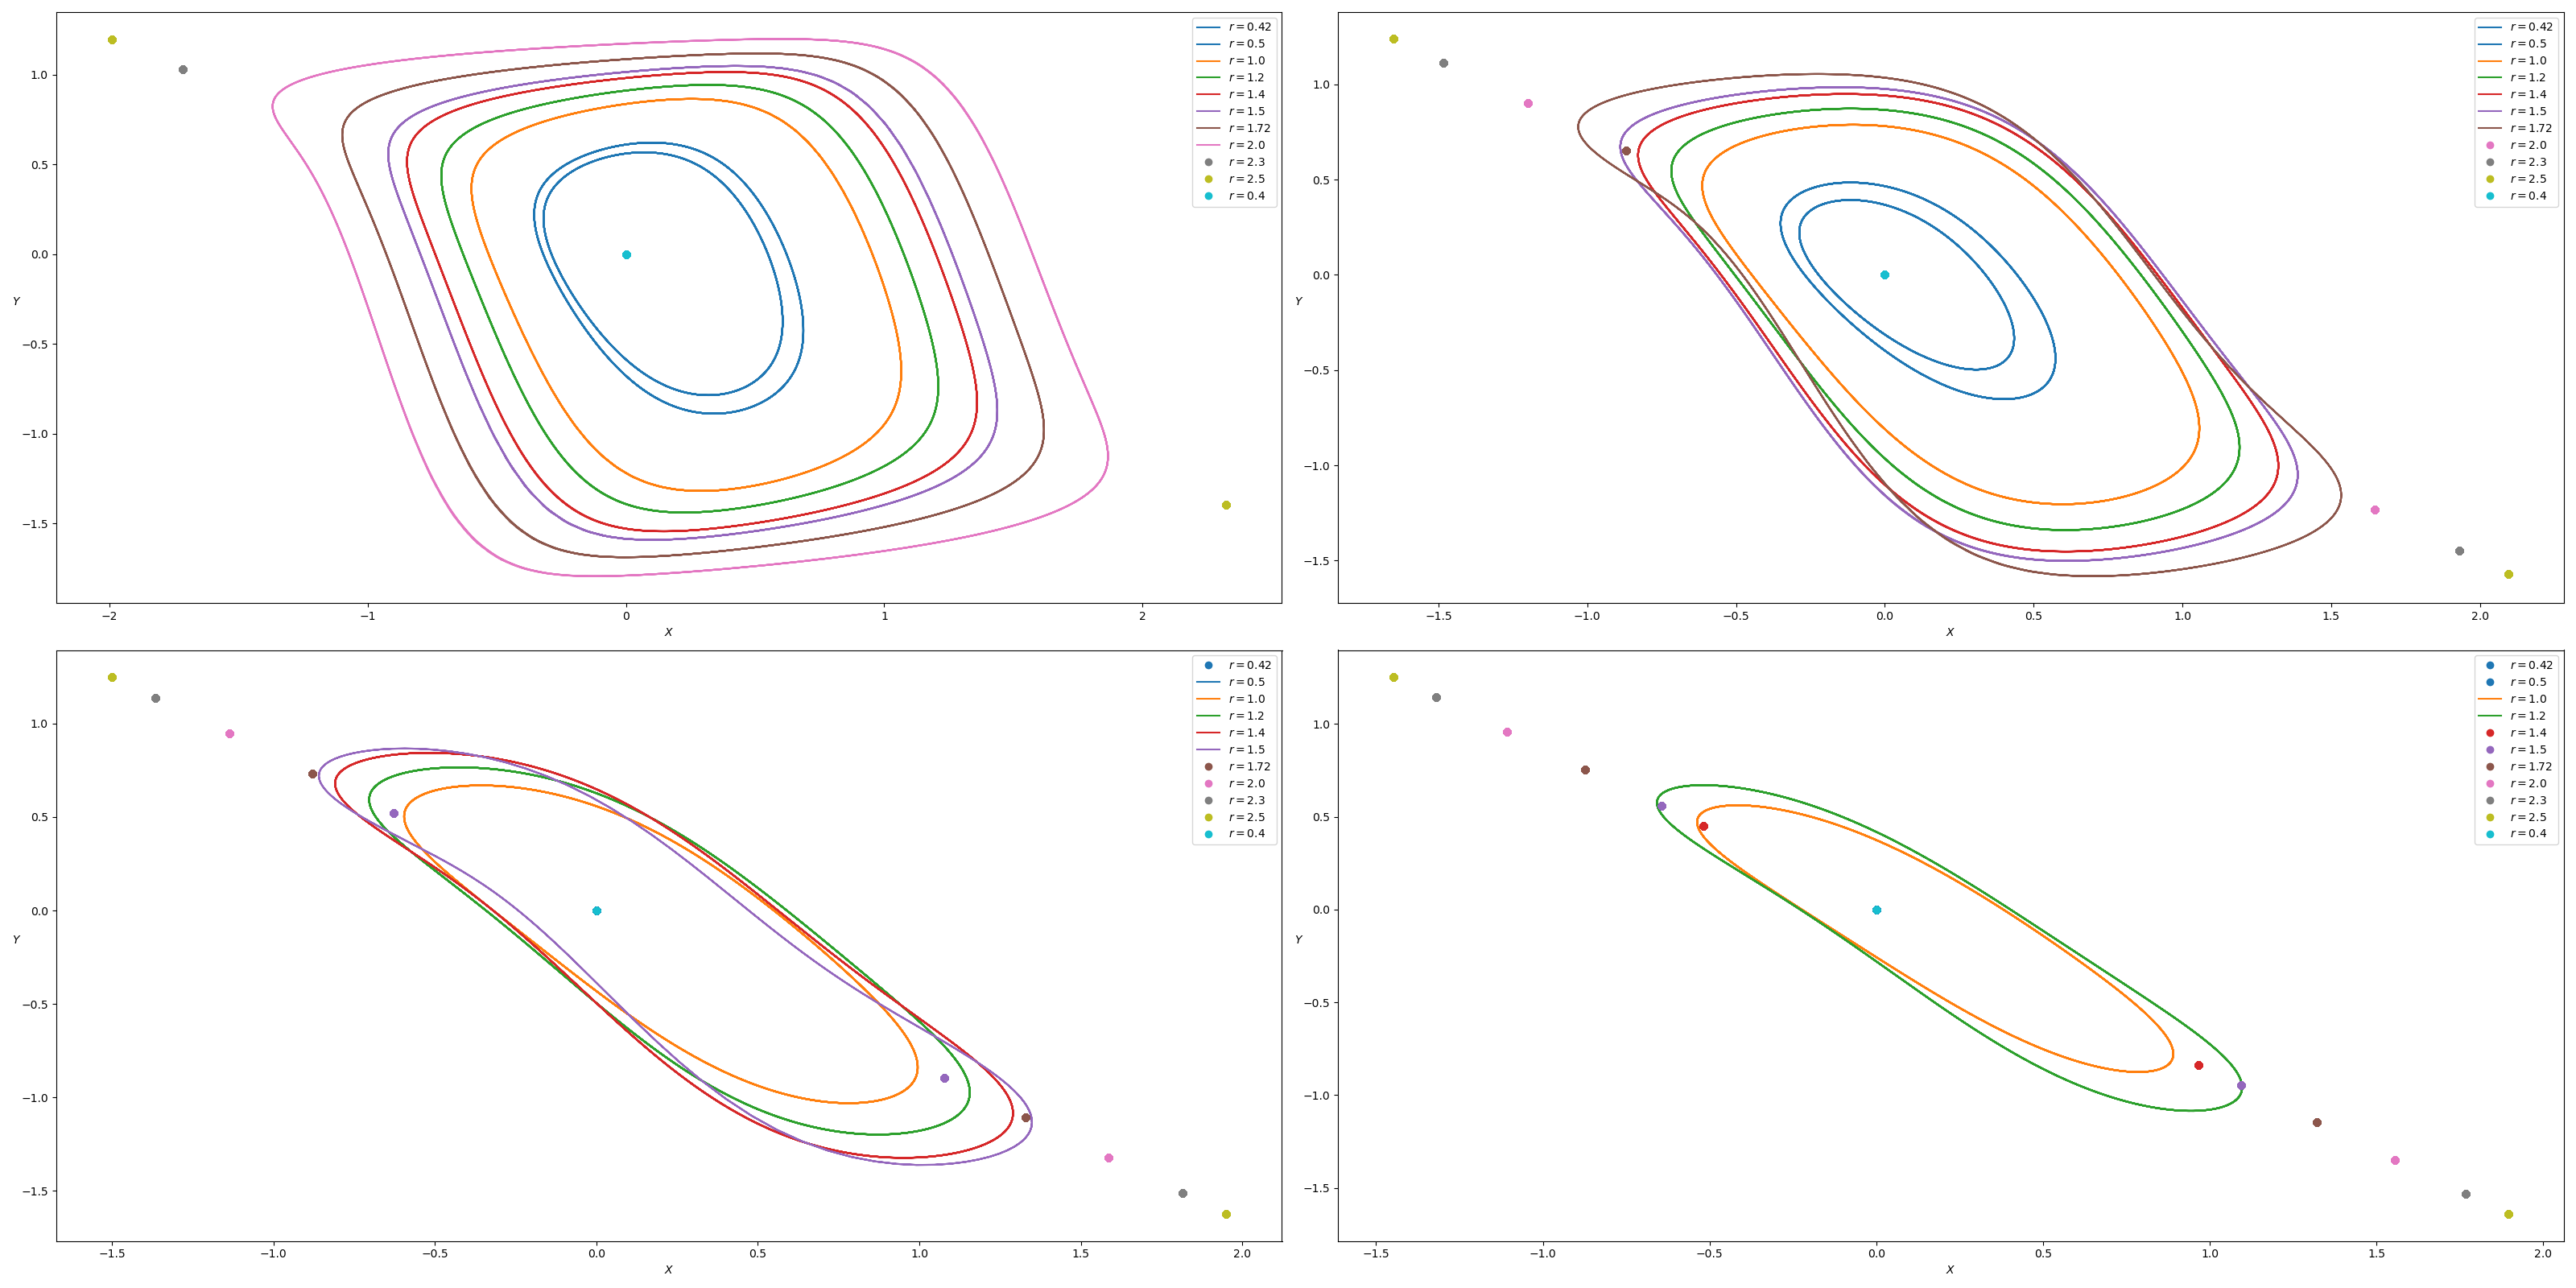
\includegraphics[width=\textwidth, height=\textheight,keepaspectratio]{figures_2/adv-attractors-a.png}
	\end{figure}
\end{frame}

\begin{frame}{Deterministic Bifurcation Diagram}
	\begin{figure}
		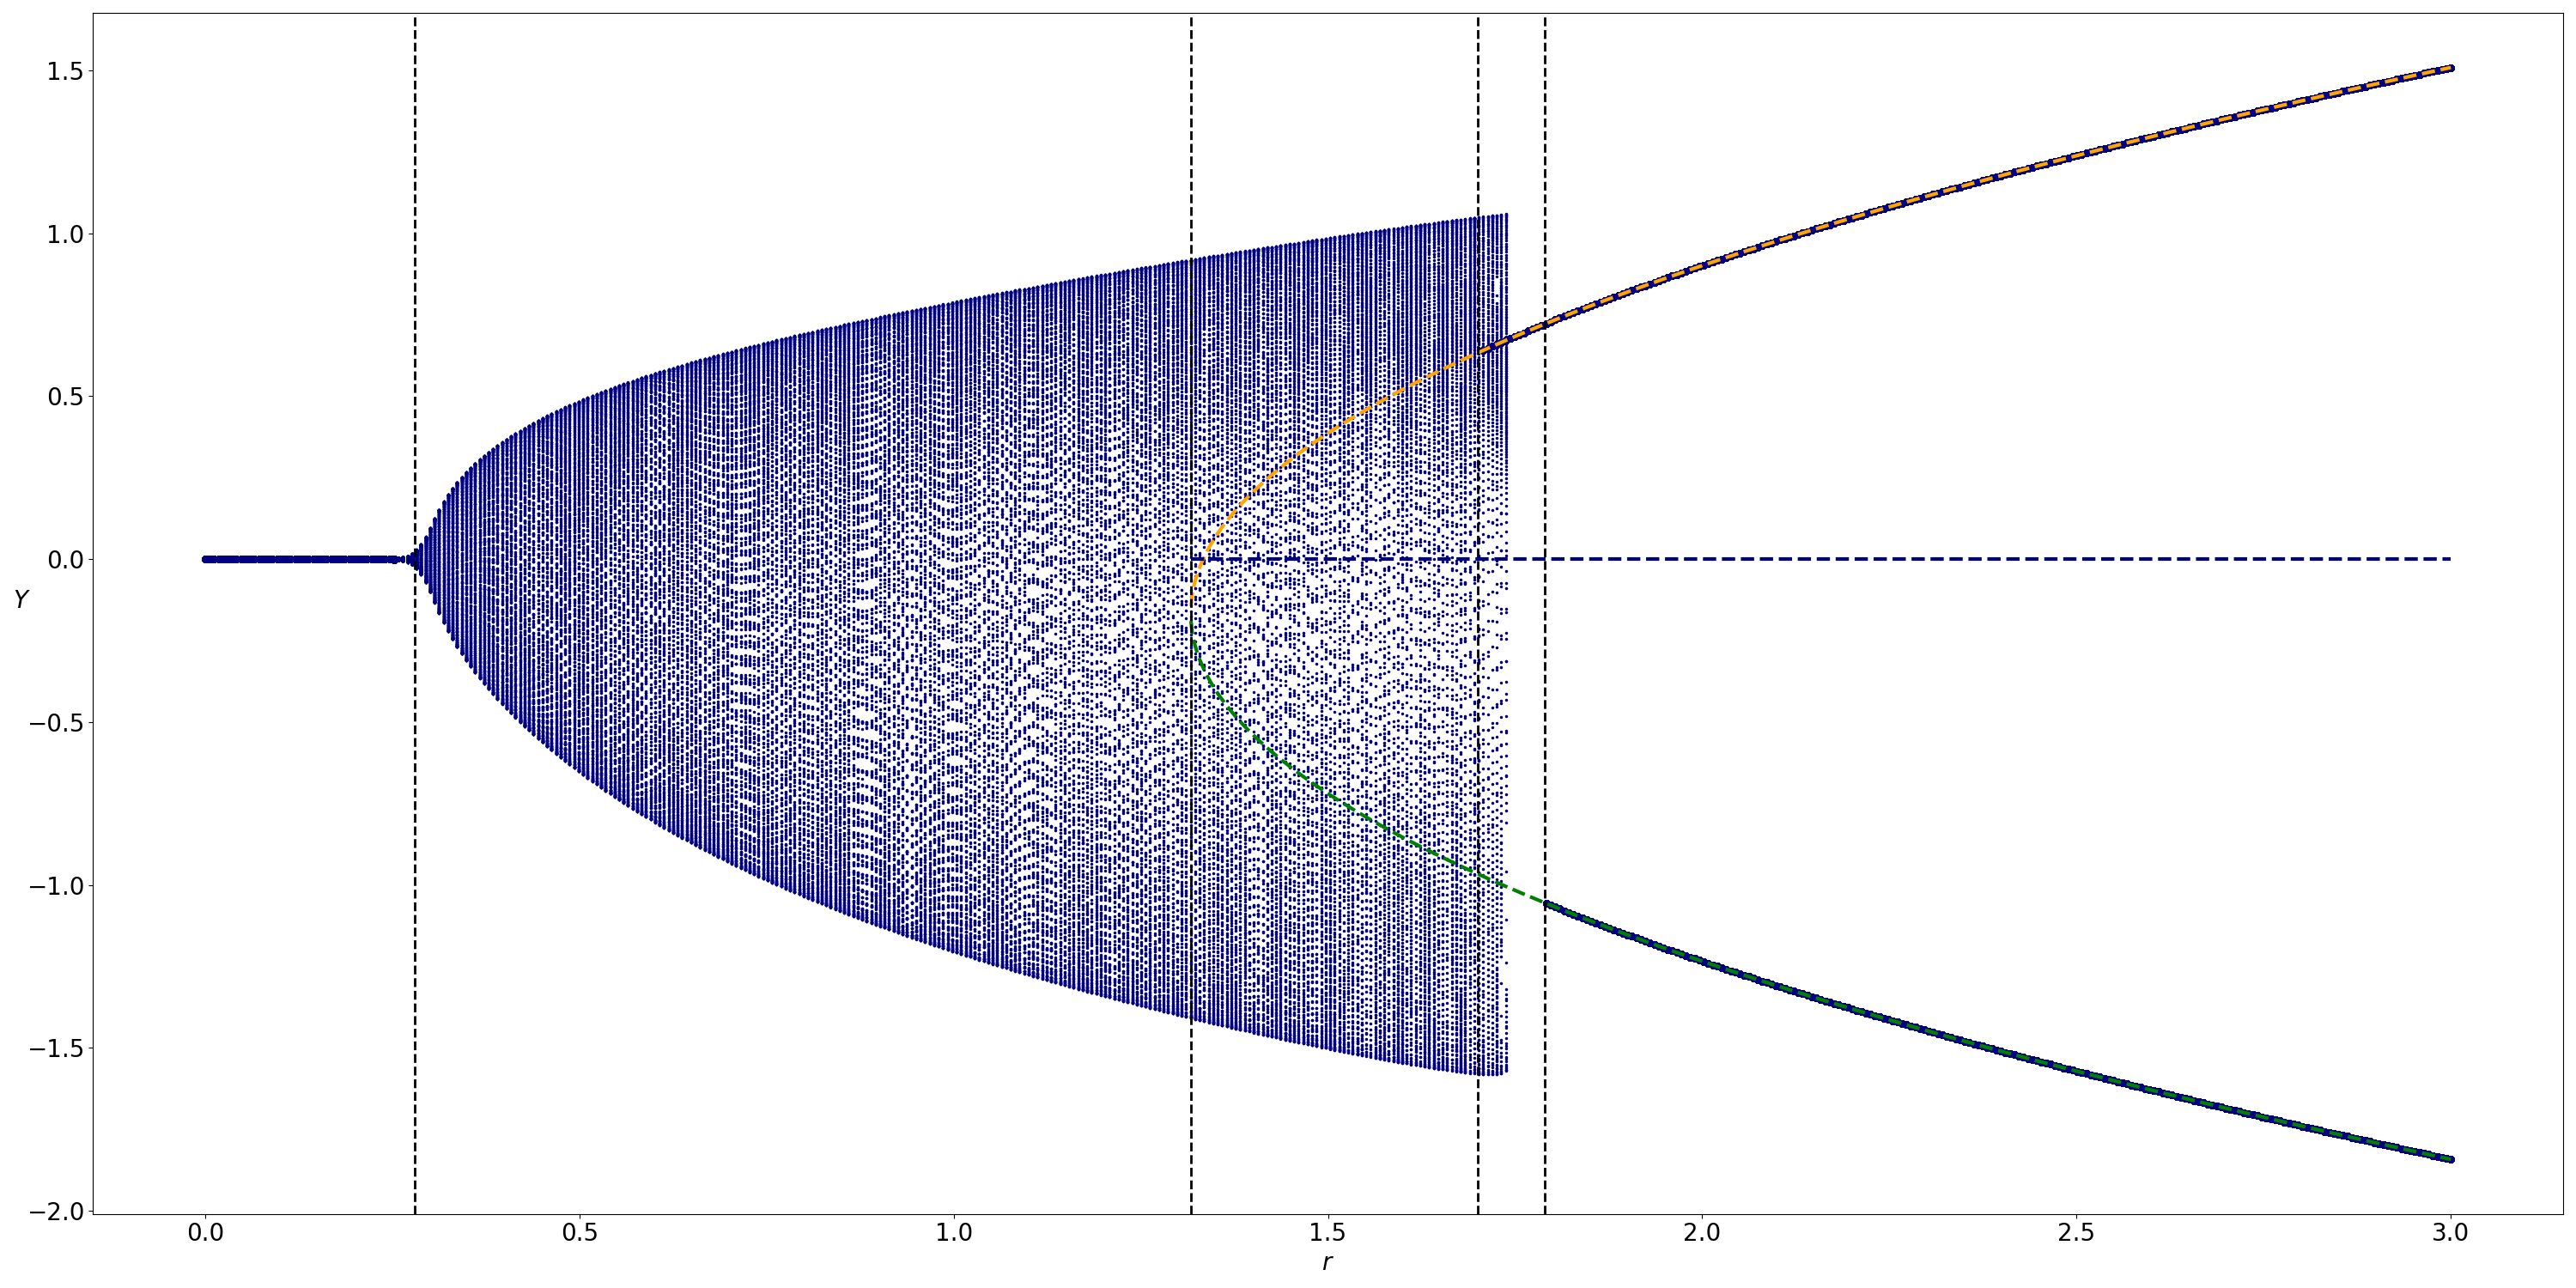
\includegraphics[width=\textwidth, height=\textheight,keepaspectratio]{figures_2/adv-noiseless-phase-portrait.png}
	\end{figure}
	Fixed for the following analysis the values of the parameters: $b=0.3, c=0.3, d=0.2, a=0.8$. \\
	Interesting thing: with this combination of parameters, the equilibrium points $E_1$ and $E_2$ 
	have the inverse stability.
\end{frame}

\begin{frame}{Stochastic system: time Behavior and Histograms}
	\begin{figure}
		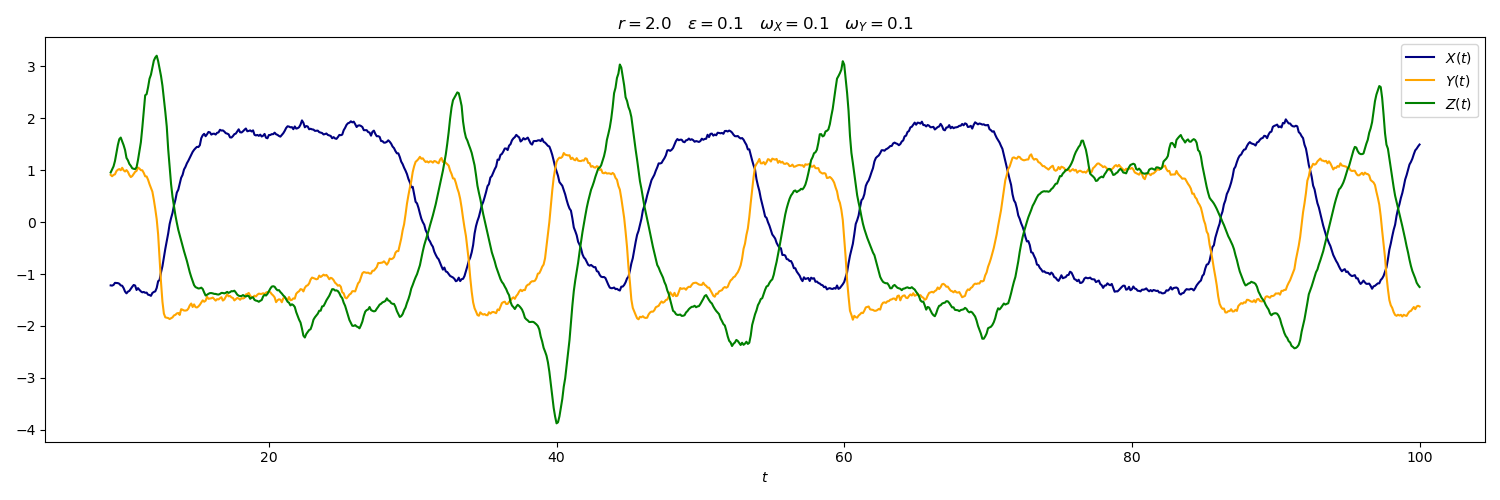
\includegraphics[width=\textwidth, height=0.52\textheight,keepaspectratio]{figures_2/r-2-eps0.1-omega0.1-time-trajectories.png}
	%\end{figure}
	%\begin{figure}
		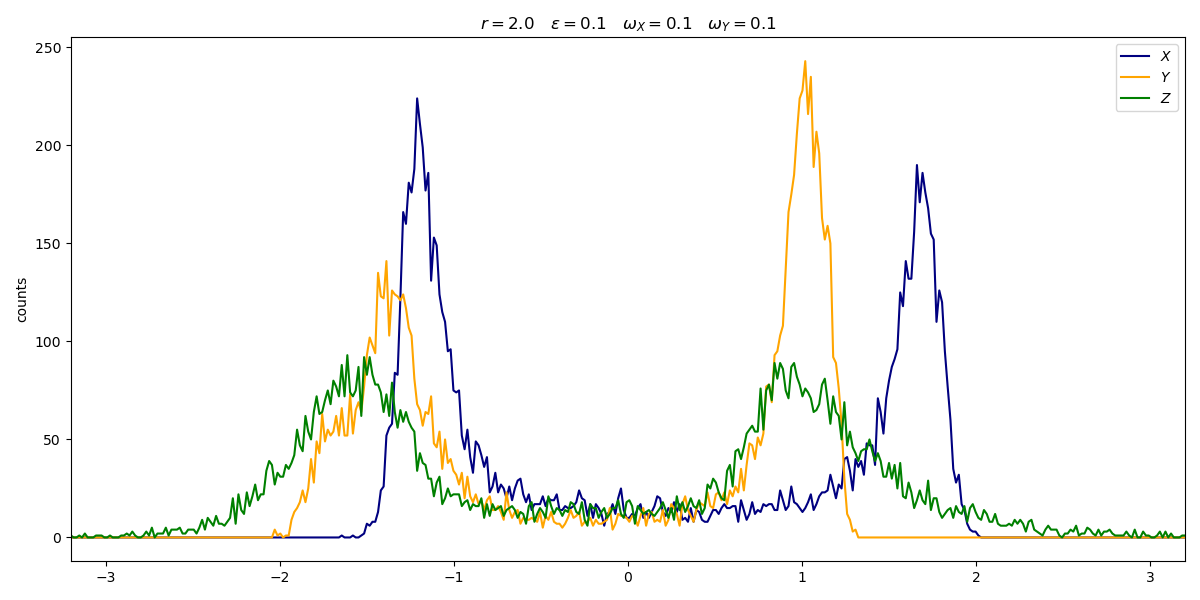
\includegraphics[width=\textwidth, height=0.52\textheight,keepaspectratio]{figures_2/r-2-eps0.1-omega0.1-hist.png}
	\end{figure}
\end{frame}

\begin{frame}{NITs}
	\begin{figure}
		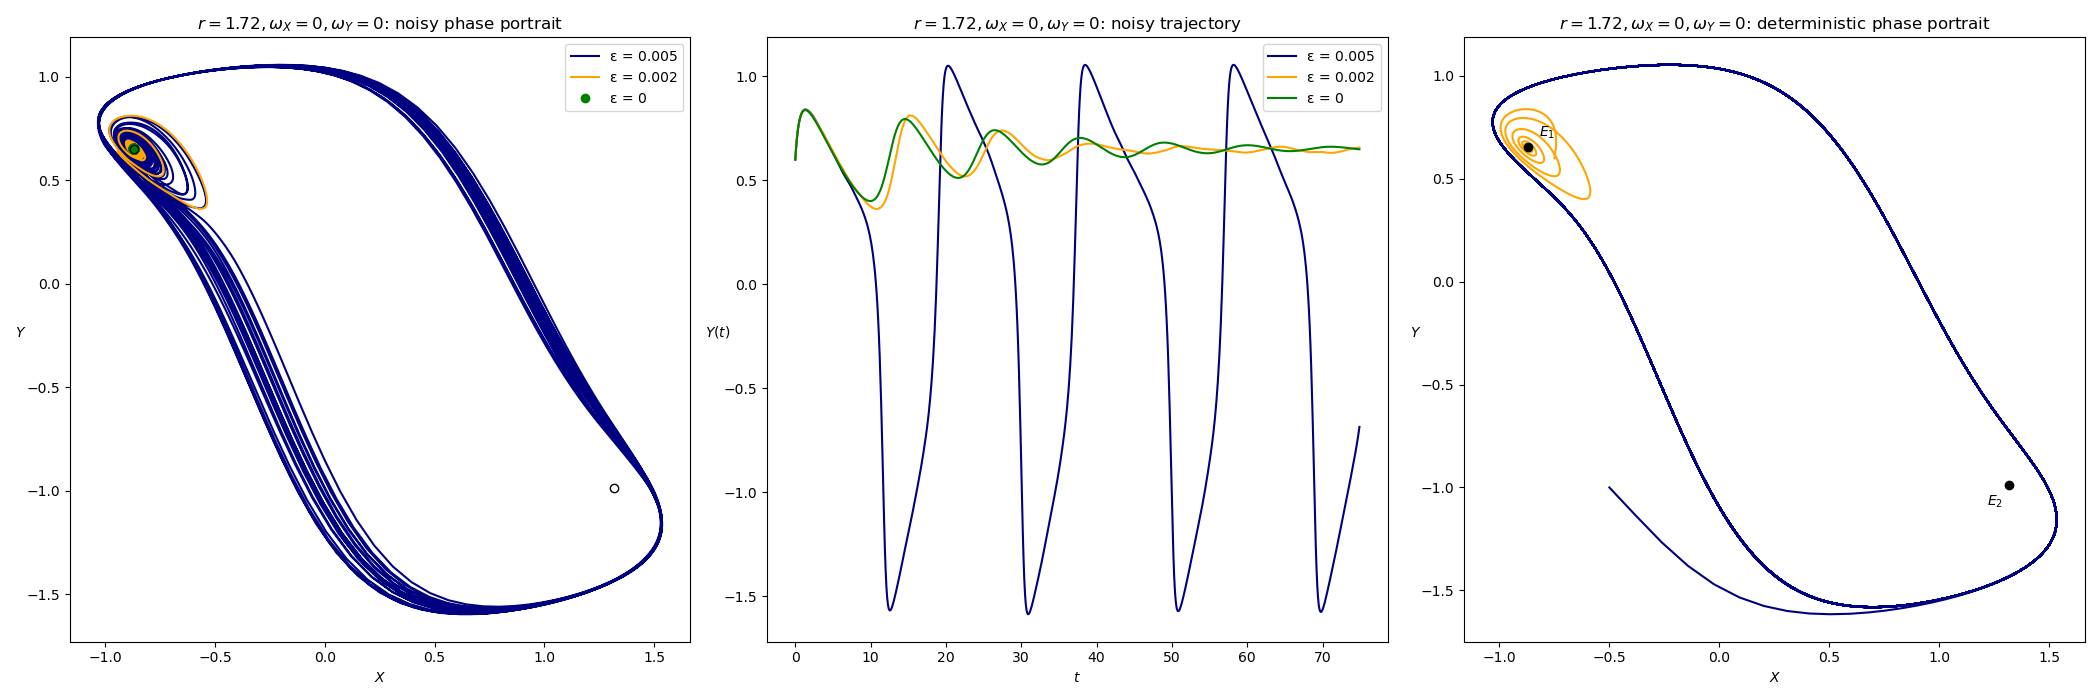
\includegraphics[width=\textwidth, height=\textheight,keepaspectratio]{figures_2/NIT-r1.72-vs-eps-adv.png}
	\end{figure}

	\begin{figure}
		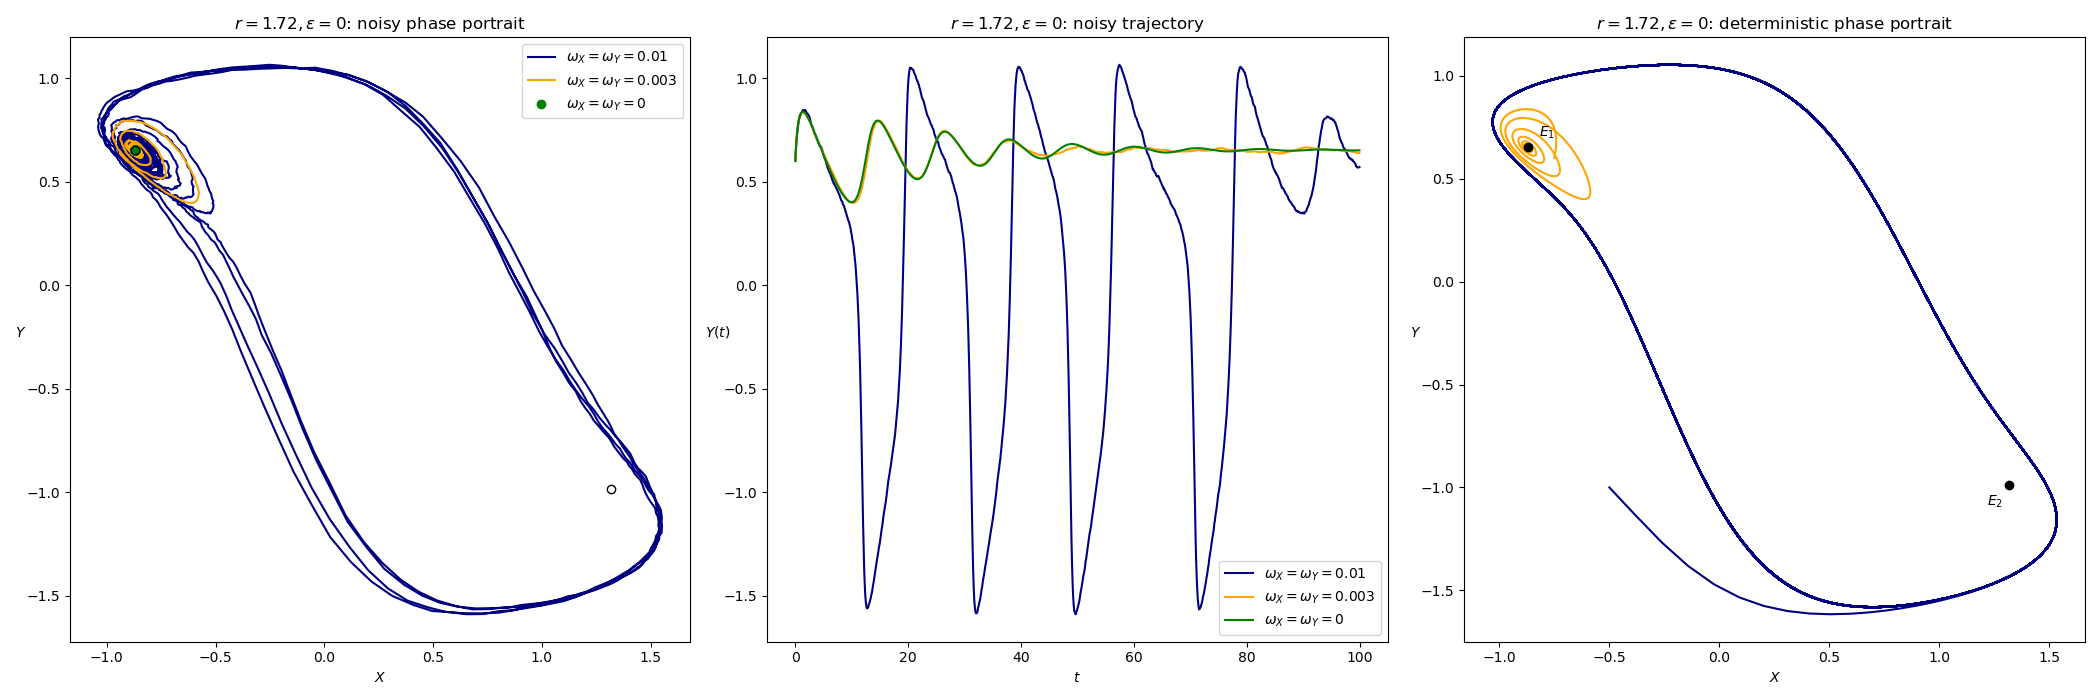
\includegraphics[width=\textwidth, height=\textheight,keepaspectratio]{figures_2/NIT-r1.72-vs-omega-adv.png}
	\end{figure}
\end{frame}

\begin{frame}{NITs}
	\begin{figure}
		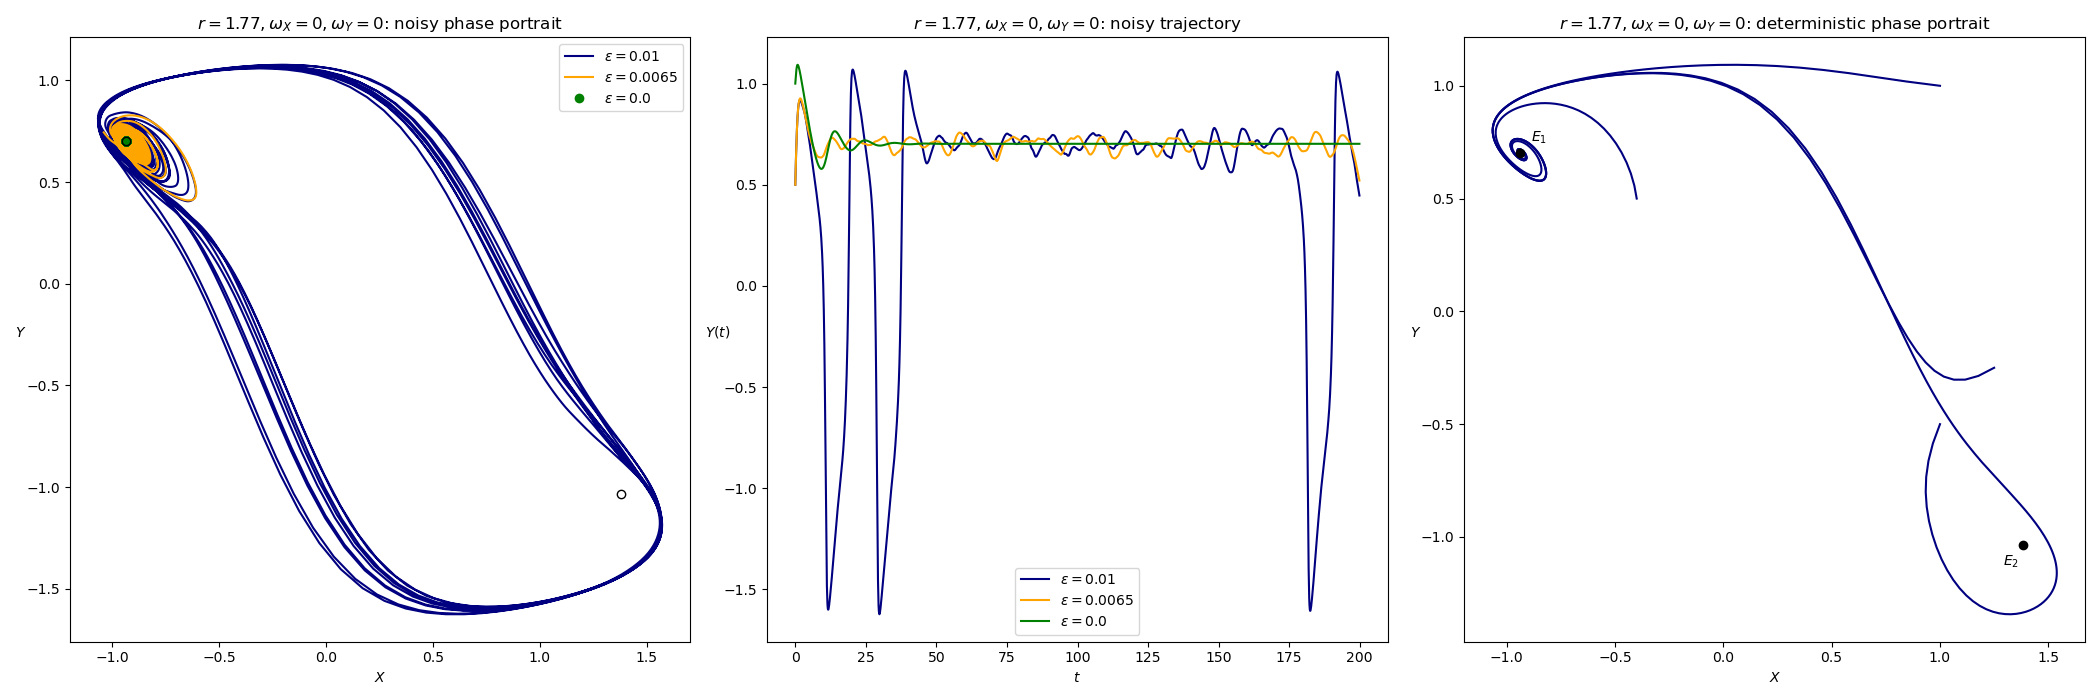
\includegraphics[width=\textwidth, height=\textheight,keepaspectratio]{figures_2/NIT-r1.77-vs-eps-adv.png}
	\end{figure}
	
	\begin{figure}
		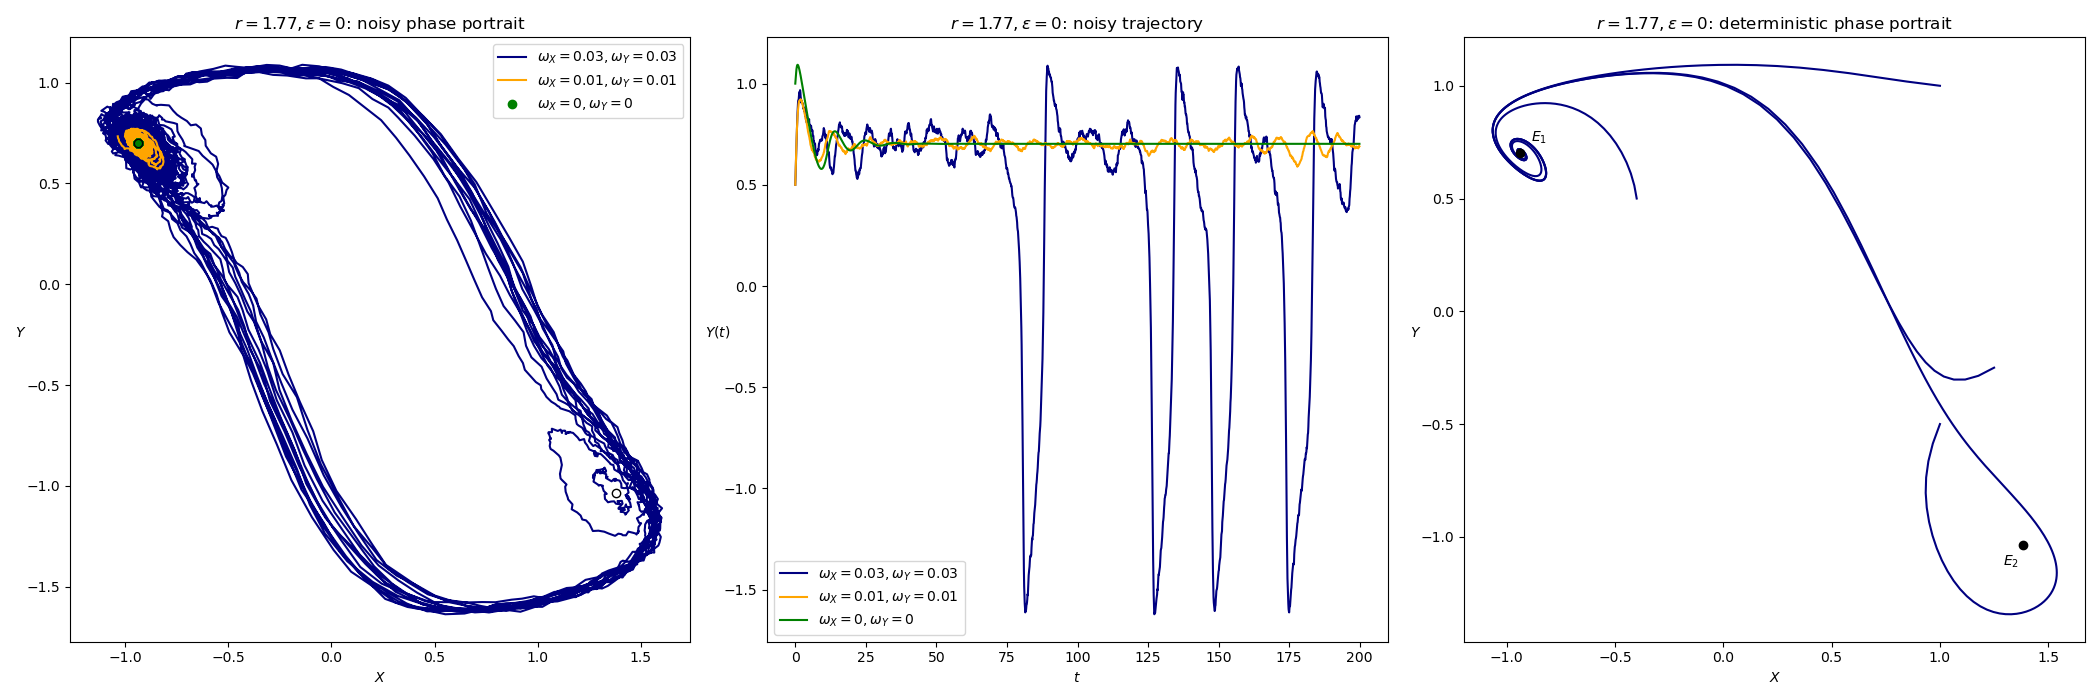
\includegraphics[width=\textwidth, height=\textheight,keepaspectratio]{figures_2/NIT-r1.77-vs-omega-adv.png}
	\end{figure}
\end{frame}

\begin{frame}{NITs}
	\begin{figure}
		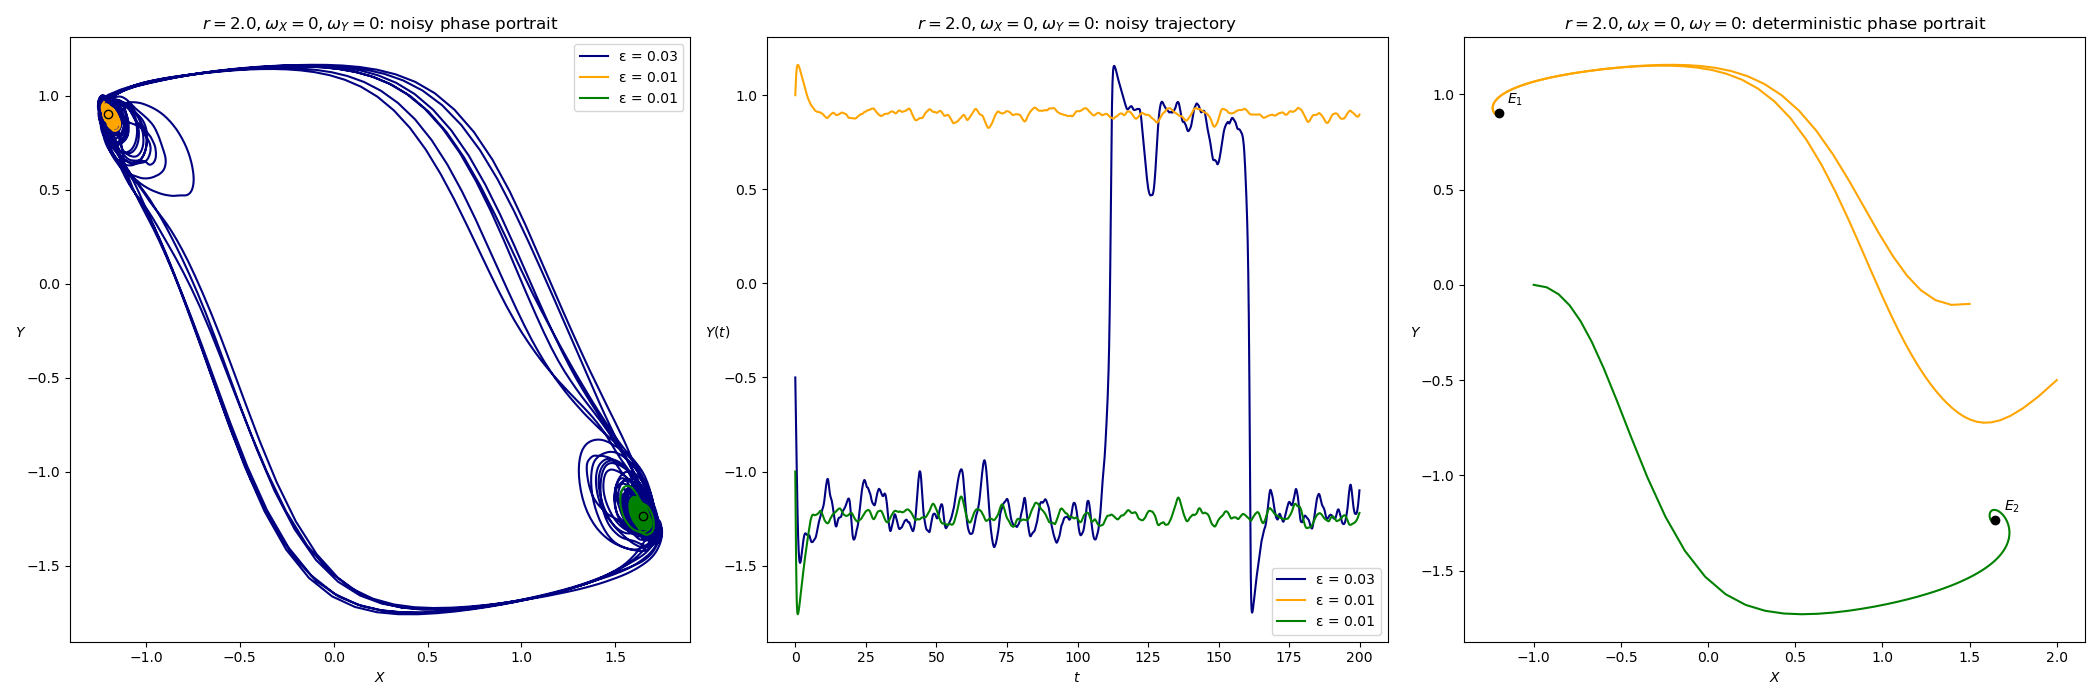
\includegraphics[width=\textwidth, height=\textheight,keepaspectratio]{figures_2/NIT-r2-vs-eps-adv.png}
	\end{figure}
	
	\begin{figure}
		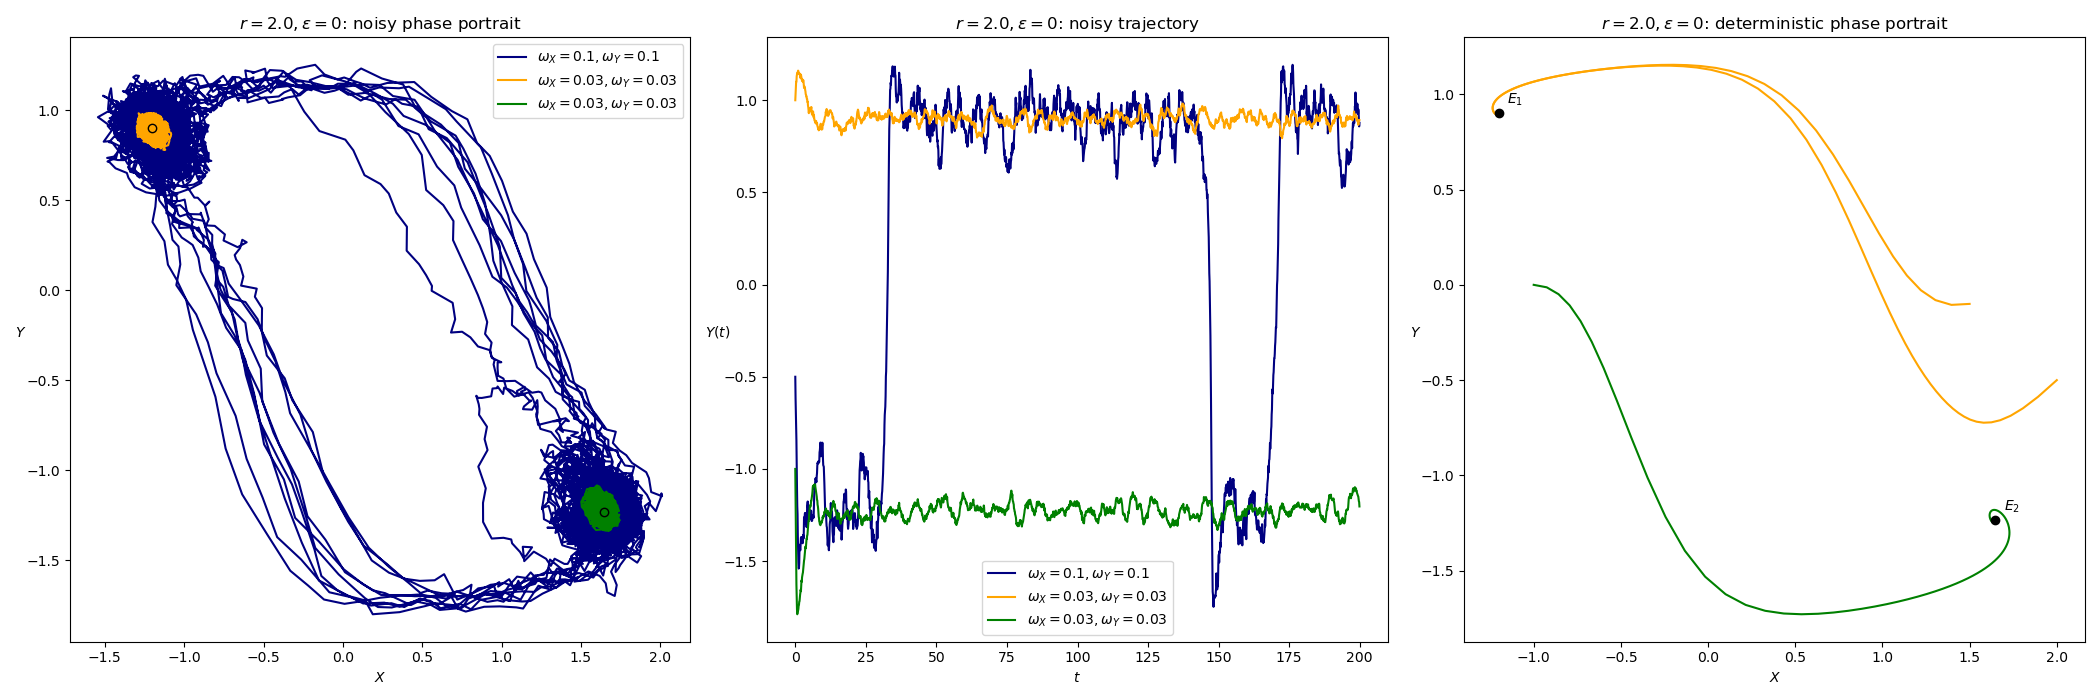
\includegraphics[width=\textwidth, height=\textheight,keepaspectratio]{figures_2/NIT-r2-vs-omega-adv.png}
	\end{figure}
\end{frame}

\begin{frame}{NITs}
	Some considerations on NITs in this case....
\end{frame}

\begin{frame}{NITs}
	\begin{figure}
		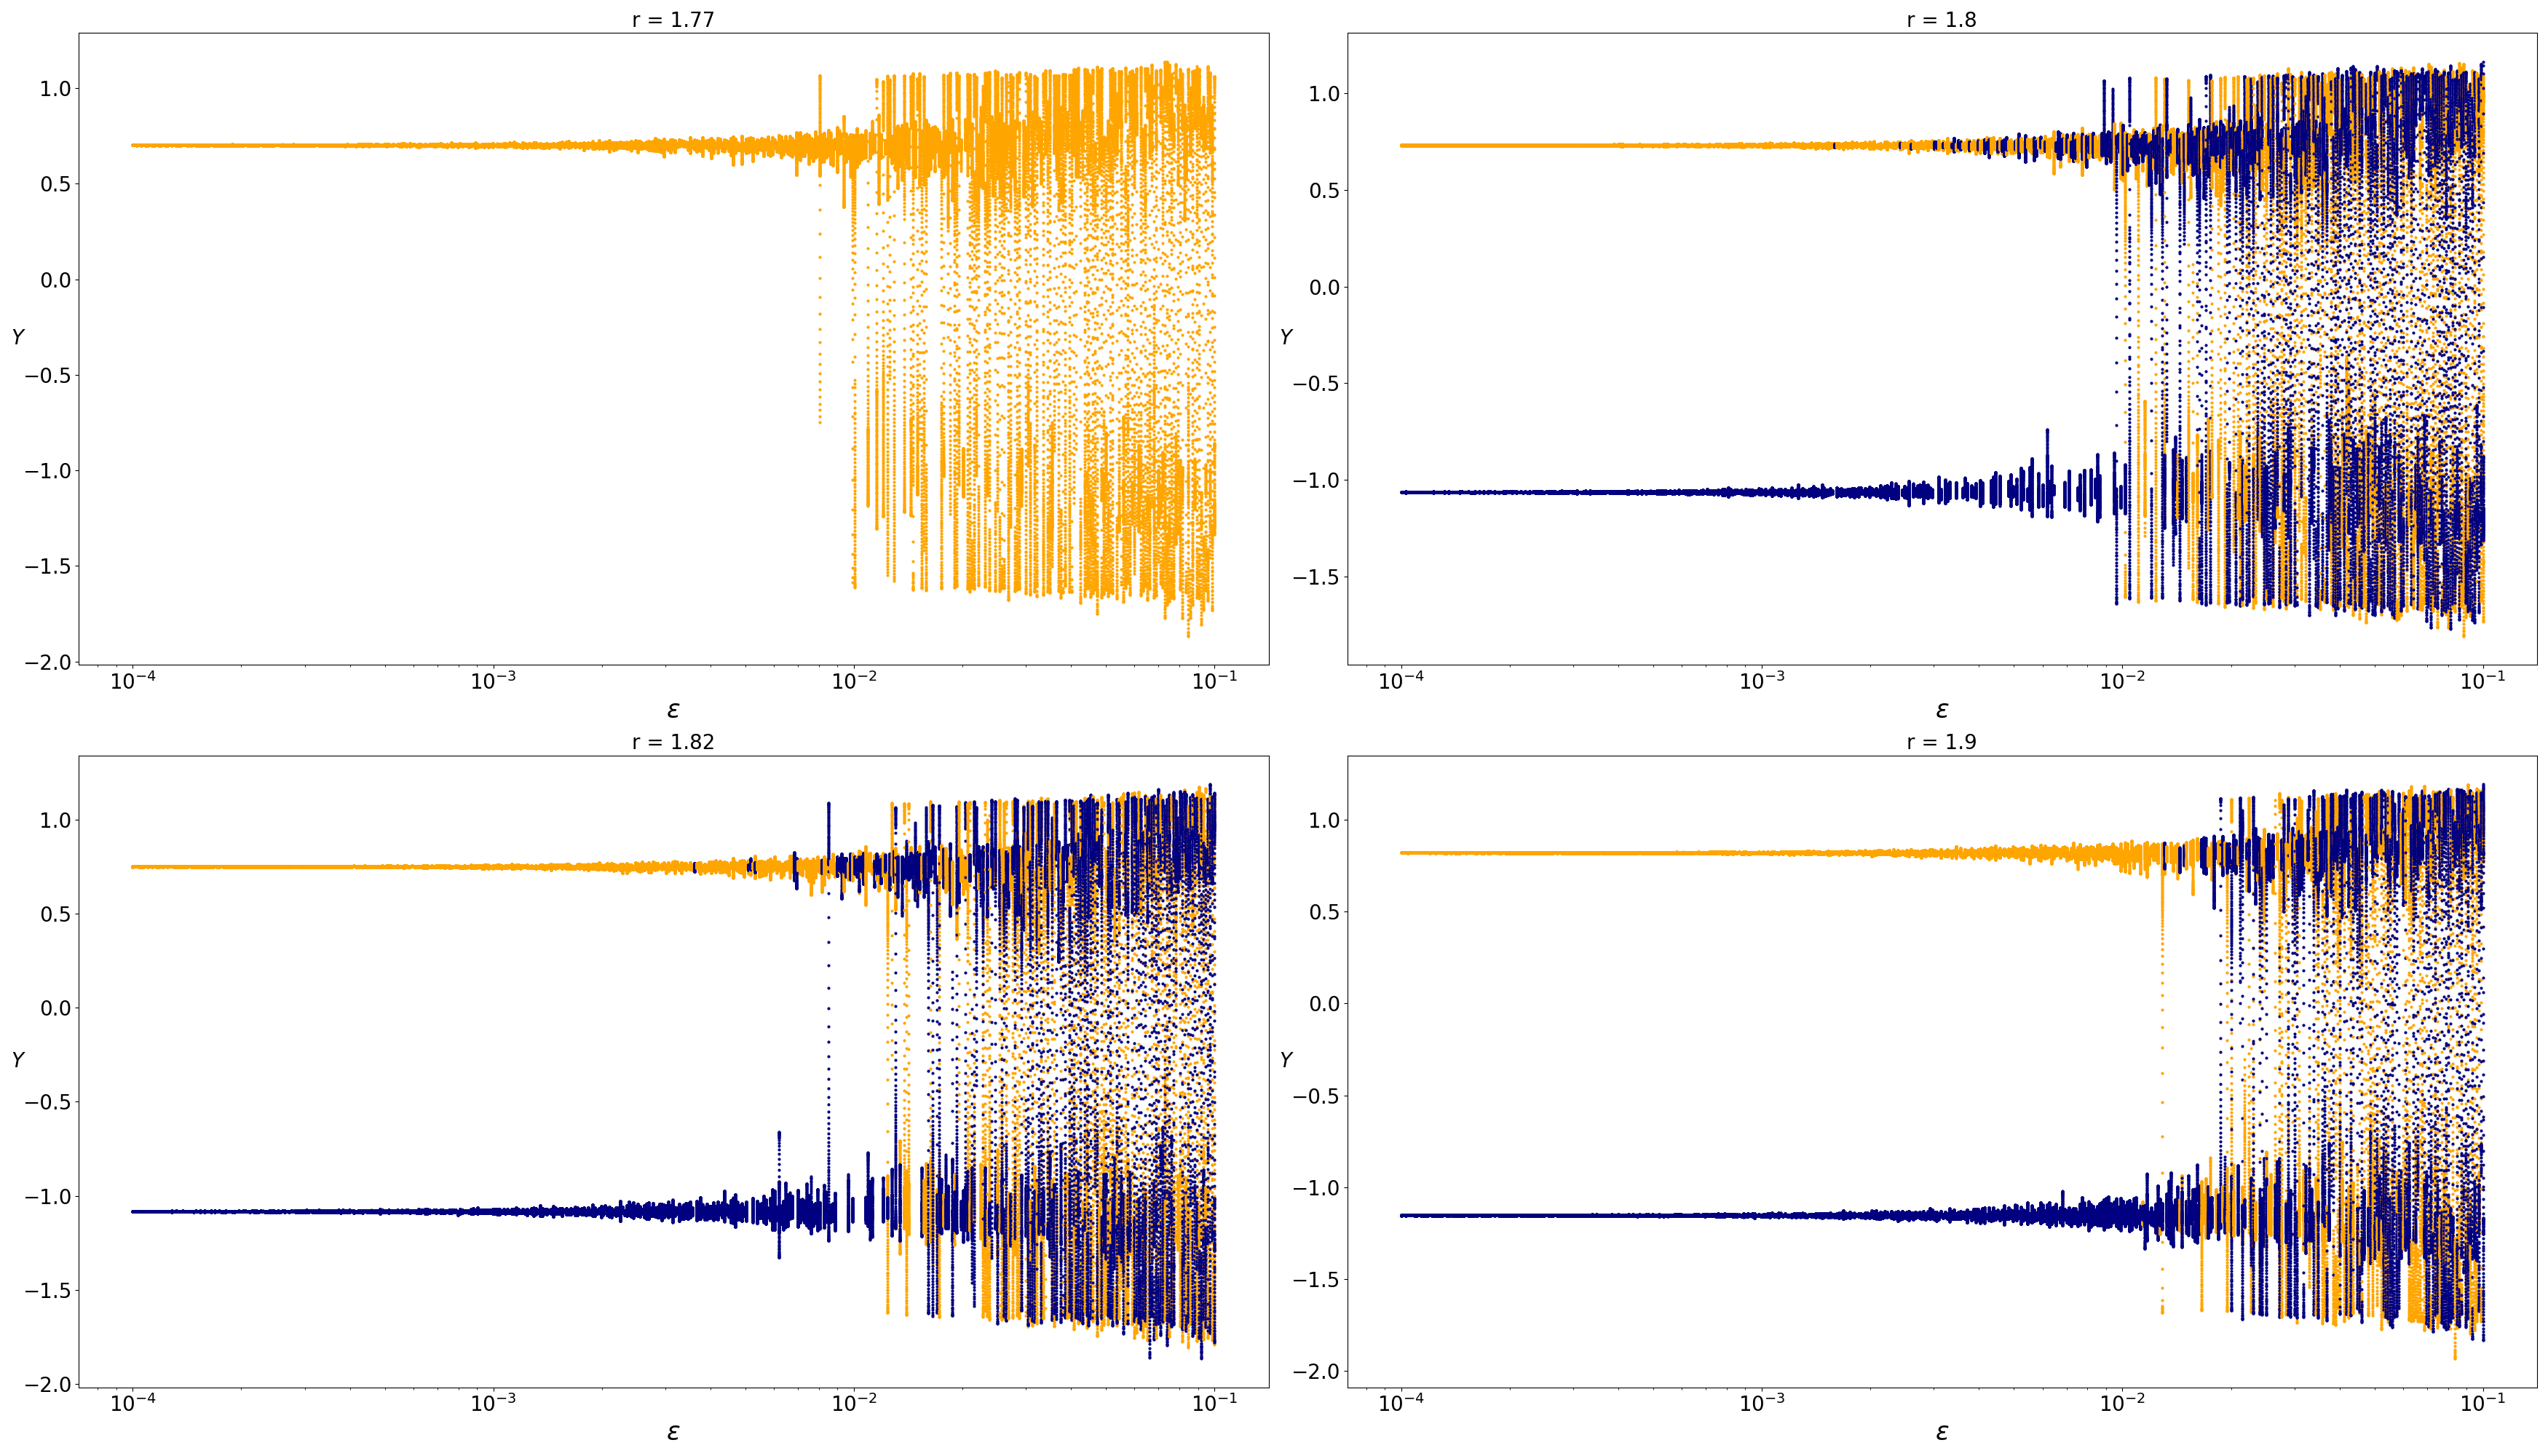
\includegraphics[width=\textwidth, height=\textheight,keepaspectratio]{figures_2/adv-NITvseps1.png}
	\end{figure}
\end{frame}

\begin{frame}{NITs}
	\begin{figure}
		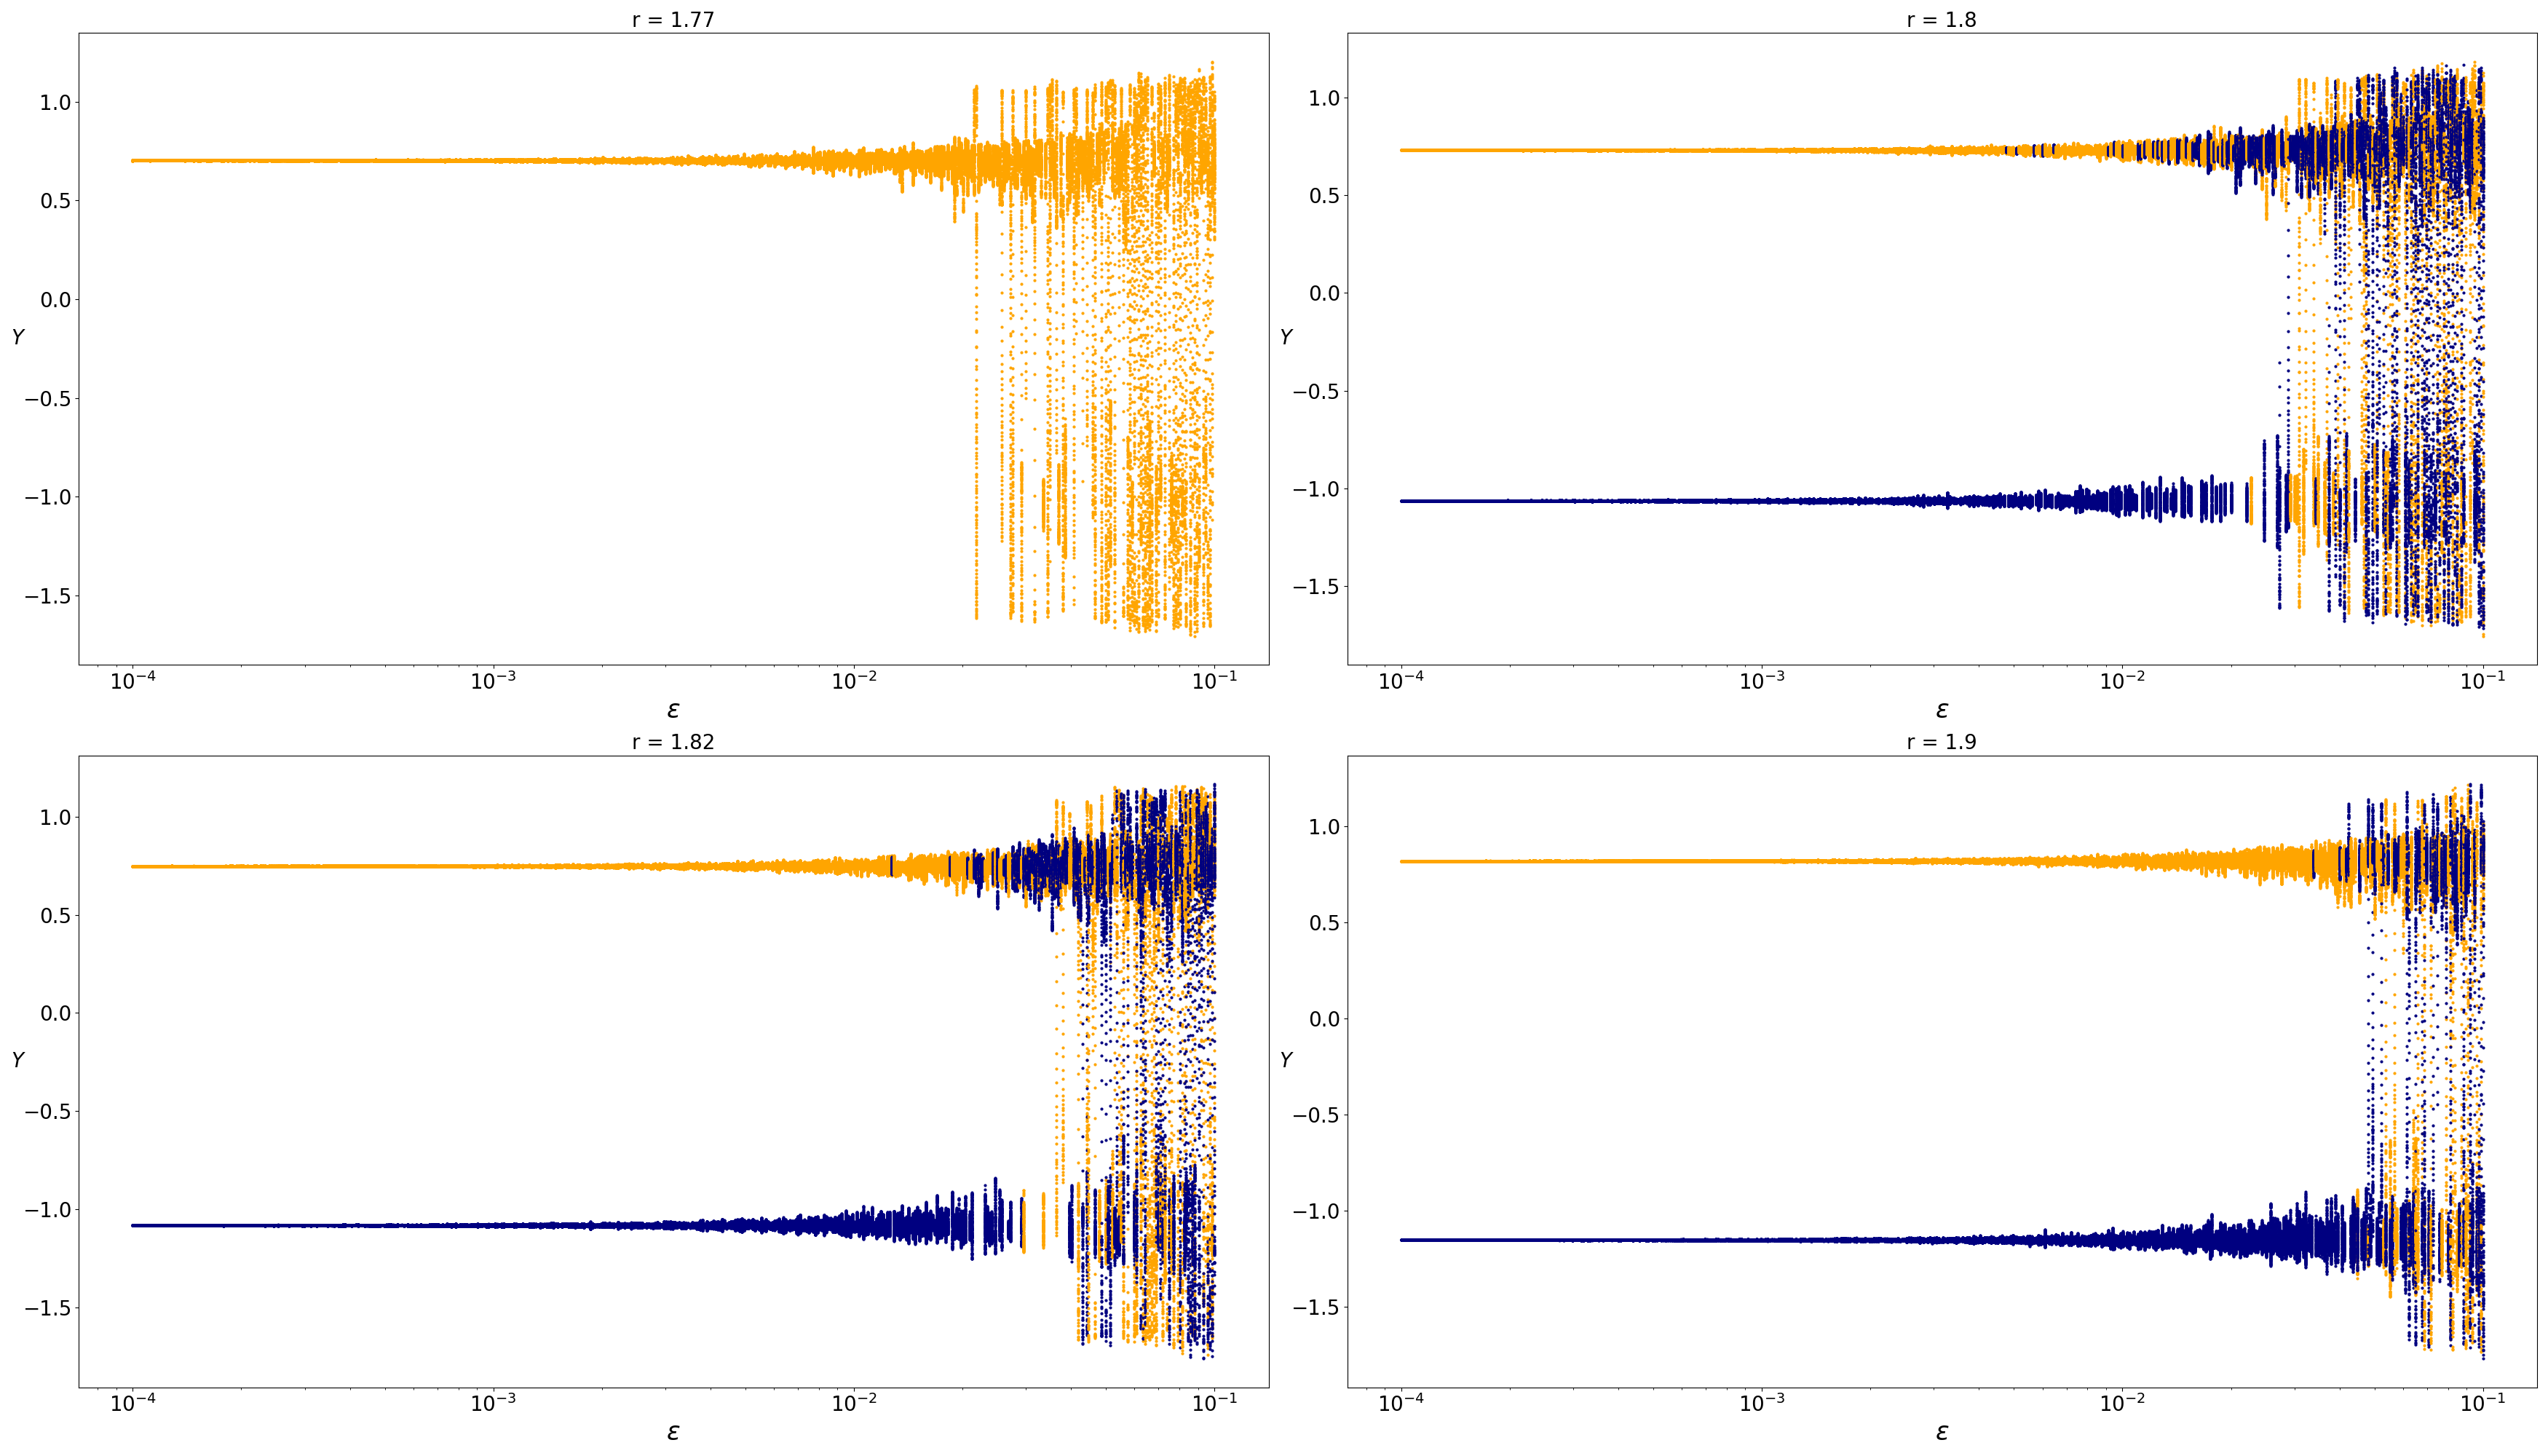
\includegraphics[width=\textwidth, height=\textheight,keepaspectratio]{figures_2/adv-NITvsomega1.png}
	\end{figure}
\end{frame}


\end{document}